\documentclass[11pt,a4paper]{article}
% Encoding and language
\usepackage[utf8]{inputenc}
\usepackage[english]{babel}
% Colors
\usepackage[usenames,dvipsnames]{color}
\usepackage{colortbl}
% Paper size and margins
%\usepackage{rotating}
\usepackage{pdflscape}
%\usepackage[a4paper,showframe]{geometry}
\usepackage{vmargin}
\setmarginsrb{2cm}{2cm}{2cm}{2cm}{0cm}{0cm}{0cm}{1.5cm}
\usepackage{pdflscape}
\usepackage{afterpage}
% Indenting
\usepackage{indentfirst}
%\setlength{\parindent}{1cm}
\setlength{\parskip}{0.5cm}
% Symbols
\usepackage{amsmath}
\usepackage{amsfonts}
\usepackage{amssymb}
% Equations
\usepackage{eulervm} % upright font in eqns (Palatino)
\usepackage{cool}
\usepackage{mathtools} % for arrows
\renewcommand{\theequation}{R\arabic{equation}}
% References
\usepackage{natbib}
\bibliographystyle{apalike}
% Hyperlinks and labels
%\usepackage{showkeys}
\usepackage[linktocpage=true,plainpages=false,pdfpagelabels=false]{hyperref}
\definecolor{citecolor}{rgb}{0.2,0.7,0.9}
\definecolor{urlcolor}{rgb}{0,0,1}
\hypersetup{
    colorlinks, linkcolor={Blue},
    citecolor={Blue}, urlcolor={Black}
}
% Figures
\usepackage{subcaption}
\usepackage{alphalph}
\usepackage{tikz}
\usetikzlibrary{shapes,arrows}
\usetikzlibrary{positioning}
\usetikzlibrary{calc}
\usepackage{epstopdf}
% Tikz styles
\tikzstyle{reg} = [rounded rectangle, text width=2cm, fill=black!5, align=center, anchor=west,font=\sffamily\Large\bfseries, minimum height=1cm, inner sep=0]
\tikzstyle{rad} = [rounded rectangle, draw=none, text width=2cm, fill=red!10, align=center, anchor=west,font=\sffamily\Large\bfseries, minimum height=1cm, inner sep=0]
\tikzstyle{long} = [rounded rectangle, draw=none, text width=3.5cm, fill=black!5, align=center, anchor=west,font=\sffamily\Large\bfseries, minimum height=1cm, inner sep=0]   
\tikzstyle{add} = [scale=1.5, draw=none,fill=none,align=center]
\tikzstyle{emp} = [draw=none,fill=none]
\tikzstyle{ar} = [->,draw=black!70,line width=2]
\tikzstyle{ln} = [-,draw=black!70,line width=2]
% Title etc
\newcommand{\mytitle}{Investigation of the relationship between tropospheric ozone production efficiency and carbon bond emissions}
\newcommand{\authorname}{Maria Zamyatina}
\newcommand{\authornumber}{Student No: 100106685}
\newcommand{\degname}{Master of Science}
\newcommand{\univname}{University of East Anglia}
\newcommand{\univaddr}{University Plain \\ Norwich NR47TJ UK}
\newcommand{\depname}{School of Environmental Sciences}
\newcommand{\mydate}{\the\year}
%% Remove author and date from the maketitle command
%\makeatletter
%\renewcommand{\@maketitle}{
%\newpage
% \null
% \vskip 2em%
% \begin{center}%
%  {\LARGE \@title \par}%
% \end{center}%
% \par} \makeatother

% PDF meta-data
\hypersetup{pdftitle={\mytitle}}
\hypersetup{pdfauthor=\authorname}

\title{\mytitle}
% =========================================================================
\begin{document}

\thispagestyle{empty}
\vskip 3cm
\begin{center}
    {\Huge\bfseries\sf \mytitle \par}
    \vskip 1cm
    \sf by
    \vskip 1cm
    \large \sf \authorname \\
    \sf \authornumber
\end{center}

\begin{center}
	\large \sf Thesis presented in part-fulfilment of the degree of \degname \\ in accordance with the regulations of the \univname
\end{center}

\vskip 5cm

\begin{minipage}{0.4\textwidth}
\begin{flushleft} 
\large \sf 
\depname \\
\univname \\
\univaddr
\vskip 0.5cm
\copyright~\mydate~\authorname
\end{flushleft}
\end{minipage}

%\vskip 0.2cm

\begin{minipage}{\textwidth}
\begin{flushleft}
%\noindent
\sf This copy of the dissertation has been supplied on condition that anyone who consults it is understood to recognise that its copyright rests with the author and that no quotation from the dissertation, nor any information derived there from, may be published without the author's prior written consent. Moreover, it is supplied on the understanding that it represents an internal University document and that neither the University nor the author are responsible for the factual or interpretative correctness of the dissertation.
\end{flushleft}
\end{minipage}

\vfill

\newpage

\tableofcontents
\newpage

\begin{abstract}
Abstract.
\end{abstract}

\section{Introduction} \label{sec:intro}
The Earth’s atmosphere is the recipient of a vast range of chemical compounds emitted by natural and anthropogenic sources. The oxidation of these compounds is the main process taking place in the atmosphere that keeps their concentrations at levels that do not distort the chemical balance of the atmosphere \citep{Prinn2003}. In other words, oxidation is a removal 'cleansing' mechanism for these compounds (various pollutants and greenhouse gases), and its rate is often referred to as the oxidizing capacity of the atmosphere. This capacity depends mainly on two factors: climate and the global burden of the principal oxidants such as ozone ($O_3$), the hydroxyl radical ($OH$) and hydrogen peroxide ($H_2O_2$) \citep{Prinn2003,Thompson1992}.

\subsection{Tropospheric ozone}
Tropospheric ozone ($O_3$) plays an important role in the chemical and thermal balance of the atmosphere. Although it accounts only for about 10\% of the total ozone, it is a primary precursor to the formation of hydroxyl radicals ($OH$) which in association with hydrogen peroxide ($H_2O_2$) determines the ‘cleansing’ capacity of the atmosphere \citep{Prinn2003,Tarasick2008,Thompson1992}. On the other hand, being a source of main pollutant removal agents, ozone is an air pollutant itself. Long exposure to its high concentrations causes respiratory problems in humans and damage to sensitive plant species \citep{Fowler2008}. Last but not least characteristic of tropospheric ozone is that it is an important greenhouse gas with a current estimated radiative forcing of  $0.40\pm 0.20~Wm^{–2}$ which is approximately one fifth of the $CO_2$ radiative forcing \citep{Hartmann2013,Myhre2013}. Due to these reasons a considerable interest in quantifying tropospheric ozone concentrations, budget and trends exists for more than a 100 years \citep{Becker2004}.

Unlike many other air pollutants, tropospheric ozone is not directly emitted, but produced following the oxidation of carbon monoxide ($CO$), methane ($CH_4$), and nonmethane volatile compounds (nmVOCs) in the presence of nitrogen oxides (NOx) \citep{Crutzen1973,Myhre2013}. The emissions of these precursors arise from both natural and anthropogenic sources which have intensified since pre-industrial times \citep{Parrish2014,Volz1988} (Figure \ref{fig:O3observations}). Presumably it has led to roughly a doubling in background tropospheric ozone concentration \citep{Guicherit2000,Hartmann2013,Tarasick2008,Vingarzan2004}, although contribution from another major source, transport from the stratosphere, may also took place \citep{Fowler2008}. Climate is also believed to be a key driver of ozone production and destruction since the chemical reactions affecting ozone concentration are strongly dependent on such climatic factors as temperature, rainfall and humidity. Therefore in a changing climate tropospheric ozone is not anymore a local air quality issue, but is a global pollution problem \citep{Fowler2008}.

\begin{figure}[h]
\includegraphics[width=\linewidth]{{./pics/Isaksen2009_O3}.png}
\caption{Observed surface ozone at different Northern Hemispheric surface stations \citep{Isaksen2009}.}
\label{fig:O3observations}
\end{figure}

According to the Intergovernmental Panel on Climate Change (IPCC) Fifth Assessment report (AR5) for present conditions (around year 2000) the global mean tropospheric ozone budget is approximately 331 Tg \citep{Myhre2013}. However, despite general agreement on how the drivers impact ozone concentrations at global and regional scales, its budget varies considerably between different modelling and observational studies \citep{Stevenson2006,Wild2007,Young2012}. Table \ref{tab:O3budget} demonstrates that the range of the global tropospheric ozone budget estimates is approximately 60 Tg which is 18\% of the mean. In terms of ozone production the variation is even higher and accounts for 28\% of the corresponding value. In that regard, two questions arise: why does the tropospheric ozone budget differ between models and observations? And secondly, why does it vary to this extent, especially in terms of production? The only way to answer these questions is to perform a rigorous investigation of the factors that drive tropospheric ozone and attribute those differences to respective factors \citep{Young2012}.

\begin{table}[h] % O3 budget
\centering
\caption{Summary of tropospheric ozone global budget model and observation estimates for present (about 2000) conditions. All uncertainties quoted as 1 standard deviation (68\% confidence interval). Adapted from \citep{Myhre2013}}
\label{tab:O3budget}
\begin{tabular}{ccl}
\hline
Burden, Tg & Production, Tg yr–1 & Reference \\
\hline
\multicolumn{3}{c}{Modelling studies} \\
$337\pm23$  & $4877\pm853$ & Young et al. (2013); ACCMIP \\
$323$	    & -	           & Archibald et al. (2011) \\
$330$	    & $4876$       & Kawase et al. (2011) \\
$312$       & $4289$       & Huijnen et al. (2010) \\
$334$       & $3826$       & Zeng et al. (2010) \\
$324$       & $4870$       & Wild and Palmer (2008) \\
$314$       & -	           & Zeng et al. (2008) \\
$319$	    & $4487$	   & Wu et al. (2007) \\
$372$	    & $5042$       & Horowitz (2006) \\
$349$	    & $4384$	   & Liao et al. (2006) \\
$344\pm39$	& $5110\pm606$ & Stevenson et al. (2006); ACCENT \\
$314\pm33$	& $4465\pm514$ & Wild (2007) (post-2000 studies) \\
\hline
\multicolumn{3}{c}{Observational studies} \\
$333$   	& -	           & Fortuin and Kelder (1998) \\
$327$	    & -	           & Logan (1999) \\
$325$	    & -	           & Ziemke et al. (2011); 60S–60N \\
$319–351$	& -	           & Osterman et al. (2008); 60S–60N \\
\hline
\end{tabular}
\end{table}

A considerable effort has been made to tackle these problems, and generally there are two possible ways of doing it. The first one implies the direct analysis of tropospheric chemical schemes used in climate-chemistry models. For example, Emmerson and Evans (2009) compared the state of the art Master Chemical Mechanism which contains approximately 5600 species and 13500 reactions \citep{Jenkin2002} with other six chemical schemes and found four significant variations between them. This approach is linked with big challenges since a modern global model is a very sophisticated representation of the climate-chemistry interactions, and therefore it is often difficult to separate influence of one reaction from another. However, even being so developed climate-chemistry models do not take into account all known chemical reactions taking place in the real troposphere. A complete representation requires many thousands of species and tens of thousands of reactions, which is beyond the numerical capabilities currently available. This significantly limits the practicable size of chemical schemes and typically involves a reduction of the number of VOCs considered and lumping the carbon from the discarded species into representative surrogates.

! add something from report!

The second way to understanding the discrepancies between models and observations is to conduct an idealised theoretical study using a conceptual model. The advantage of this approach is that such kind of models can be quite easily constructed, and more importantly can be focused on representation of a certain chemical reactions which presumably could explain the discrepancy between models and observations.

\subsubsection*{Ozone tropospheric chemistry}
%\documentclass[]{standalone}
\usepackage[utf8]{inputenc}
\usepackage[english]{babel}
\usepackage{amsmath}
\usepackage{amsfonts}
\usepackage{amssymb}

\usepackage{graphicx}
%\usepackage[left=2cm,right=2cm,top=2cm,bottom=2cm]{geometry}

% Figures
\usepackage{tikz}
\usetikzlibrary{shapes,arrows}
\usetikzlibrary{positioning}
\usetikzlibrary{calc}
%\usepackage{chemfig}

% Tikz styles
\tikzstyle{reg} = [rounded rectangle, text width=2cm, fill=black!5, align=center, anchor=west,font=\sffamily\Large\bfseries, minimum height=1cm, inner sep=0]
\tikzstyle{rad} = [rounded rectangle, draw=none, text width=2cm, fill=red!10, align=center, anchor=west,font=\sffamily\Large\bfseries, minimum height=1cm, inner sep=0]
\tikzstyle{long} = [rounded rectangle, draw=none, text width=3.5cm, fill=black!5, align=center, anchor=west,font=\sffamily\Large\bfseries, minimum height=1cm, inner sep=0]   
\tikzstyle{add} = [scale=1.5, draw=none,fill=none,align=center]
\tikzstyle{emp} = [draw=none,fill=none]
\tikzstyle{ar} = [->,draw=black!70,line width=2]
\tikzstyle{ln} = [-,draw=black!70,line width=2]


\begin{document}
\begin{tikzpicture}[node distance = 4cm, auto]

% Nodes: big cycle: CH4-CH302-CH3NO3-CH3O-HCHO-HO2-OH-O3
\node[reg] (ch4) {$CH_4$};
\node[add](foo1_1) at (3,-2) {};
\node[add](foo1_2) at (4,-2) {$O_2$\\$OH$};
\node[reg] (ch3o2) at (5,-4){$CH_3 O_2$};
\node[reg] (oh) at (5,4){$OH$};
\node[long] (ch3ooh) at (0,-8){$CH_3OOH$};
\node[reg] (oz1) at (0,8){$O_3$};
\node[emp] (foo2) at ($(oz1)!.5!(oh)$){};
\node[reg] (ho2) at (15,4){$HO_2$};
\node[add] (oz_up) at ($(ho2)!.5!(oh) + (0,0.5)$){$O_3$};
\node[reg] (h2o2) at (17.5,7.5){$H_2O_2$};
\node[add] (ho2_) at (16.5,6){$HO_2$};
\node[emp] (nox_top) at ($(ho2)!.5!(oh) + (0,1.5)$){};
\node[reg] (ch3o) at (15,-4){$CH_3 O$};
\node[reg] (hcho) at (20,0){$HCHO$};
\node[emp] (foo5) at (19,-2){};
\node[long] (ch3no3) at (10,-10){$CH_3 NO_3$};
\node[add] (foo1_2) at (7,-9) {$NO$};
%\node[emp] (dep1) at (11,-12){};
%\node[add] (dep1_) at (10.3,-11.3){deposition};

%Nodes: Bottom NOx cycle + misc
\node[add] (no_1) at (7,-6){$NO$};
\node[add] (no2_1) at (13,-6){$NO_2$};
\node[emp] (nox_bottom) at ($(no_1)!.5!(no2_1)+(0,2)$){};
\node[emp] (foo7) at (11.5,-7.5){};
\node[add] (hv_11) at (12,-7){$h\nu$};
\node[reg] (o3_1) at (9.25,-8.75){$O_3$};
\node[add] (o2_1) at (11.2,-7.9){$O_2$};
\node[emp] (foo3) at (16,-8){};
\node[add] (hv_12) at (15,-8.75){$h\nu$};
\node[emp] (foo4) at (19,-8){};
\node[add] (oh_) at (20,-6.5){$OH$};
\node[add] (o2_) at (18,-3){$O_2$};

%Nodes: Top NOx cycle + misc
\node[add] (no2_2) at ($(ho2)!.5!(oh)+(-3,3.5)$){$NO_2$};
\node[add] (no_2) at ($(ho2)!.5!(oh)+(3,3.5)$){$NO$};
\node[add] (hv_2) at (10,9){$h\nu$};
\node[reg] (o3_2) at (13,10.5){$O_3$};
\node[add] (o2_2) at (12.75,9.75){$O_2$};
\node[emp] (foo6) at (11.5,9.5){};

%Nodes: CO & CO2
\node[reg] (co) at ($(ho2)!.5!(oh)+(-4,-3)$){$CO$};
\node[reg] (co2) at ($(ho2)!.5!(oh)+(2,-3)$){$CO_2$};
\node[emp] (cc_o2) at ($(ho2)!.5!(oh)+(0,-2.5)$){};
\node[emp] (cc_1) at ($(ho2)!.5!(oh)+(-0.5,-1.5)$){};
\node[emp] (cc_2) at ($(ho2)!.5!(oh)+(0.5,-1.5)$){};
\node[add] (cc_o2) at ($(ho2)!.5!(oh)+(0,-2)$){$O_2$};

%Nodes: HCHO decompostion
\node[long] (co_2ho2) at (25,3){$CO~+~2HO_2$};
\node[add] (hcho_hv1) at ($(hcho)!.5!(co_2ho2)$){$h\nu$};
\node[long] (co_h2) at (25,0){$CO~+~H_2$};
\node[add] (hcho_hv2) at ($(hcho)!.5!(co_h2)+(0.25,0.25)$){$h\nu$};
\node[long] (co_ho2) at (25,-3){$CO~+~HO_2$};
\node[add] (hcho_oh) at ($(hcho)!.5!(co_ho2)+(0.25,0)$){$OH$};
%\node[long] (hno3dep) at (25,-6){\small $CO~+~HO_2~+~HNO_3$\\ deposition?};
%\node[add] (hcho_no3) at ($(hcho)!.5!(hno3dep)$){$NO_3$};

%Nodes: after decomposition HO_2 + CO_2
\node[emp] (decomp) at ($(co_2ho2)!.5!(co_ho2)+(3,0)$){};
\node[long] (decomp2) at ($(decomp)+(2,0)$){$HO_2~+~CO_2$};
\node[add] (decomp_oh) at ($(decomp)+(1,0.5)$){$OH$};

% Connections: big cycle
\draw[ln] (oh.west) to [out=180,in=90](foo1_1.center);
\draw[ln] (ch4.east) to [out=0,in=90](foo1_1.center);
\draw[ar] (foo1_1.center) to [out=270,in=180](ch3o2.west);
\draw[ar] (ch3o2) to (ch3ooh);
\node[add](foo1) at ($(ch3o2)!.5!(ch3ooh) + (-1,0)$) {$HO_2$};
%\draw[ar] (oz1) to node[right]{$h\nu$}(foo2.north west);
\draw[ar] (oz1) to (oh);
\node[add] (o3_to_OH) at ($(oz1)!.5!(oh) + (0.5,0.5)$){$h\nu$\\ $H_2O$};
%\draw[ar] (foo2.south east) to node[right]{$H_2O$}(oh);
\draw[ar] (ho2) to (h2o2);
\draw[ln] (ho2.north west) to [out=135,in=0](nox_top.center);
\draw[ar] (nox_top.center) to [out=180,in=45](oh.north east);
\draw[ar] (ho2) to (oh);
\draw[ln] (ch3o2) to (nox_bottom.center);
\draw[ar] (nox_bottom.center) to (ch3o);
\draw[ar] (ch3o2.south) to [out=270,in=180](ch3no3.west);
\draw[ln] (ch3o.east) to [out=0,in=270](foo5.center);
\draw[ar] (foo5.center) to [out=90,in=0](ho2.east);
\draw[ar] (foo5.center) to [out=90,in=180](hcho.west);

% Connections: bottom NOx cycle + misc
\draw[ln] (no_1.north) to [out=90,in=180](nox_bottom.center);
\draw[ar] (nox_bottom.center) to [out=0,in=90](no2_1.north);
\draw[ln] (no2_1.south) to [out=270,in=0](foo7.center);
\draw[ar] (foo7.center) to [out=180,in=90](o3_1.north);
\draw[ar] (foo7.center) to [out=180,in=270](no_1.south);
\draw[ln] (ch3no3.east) to [out=0,in=270](foo3.center);
\draw[ar] (foo3.center) to [out=90,in=270](ch3o.south);
\draw[ar] (foo3.center) to [out=90,in=0](no2_1.east);
\draw[ln] (ch3no3.east) to [out=0,in=270](foo4.center);
\draw[ar] (foo4.center) to [out=90,in=270](hcho.south);
\draw[ar] (foo4.center) to [out=90,in=0](no2_1.east);
%\draw[ar] (ch3no3.south) -- (dep1.center);

% Connections: top NOx cycle
\draw[ln] (no_2.south) to [out=270,in=0](nox_top.center);
\draw[ar] (nox_top.center) to [out=180,in=270](no2_2.south);
\draw[ln] (no2_2.north) to [out=90,in=180](foo6.center);
\draw[ar] (foo6.center) to [out=0,in=90](no_2.north);
\draw[ar] (foo6.center) to [out=0,in=270](o3_2.south);

%Connections: CO & CO2
\draw[ln] (oh.south east) to [out=315,in=180](cc_1.center);
\draw[ln] (co.north east) to [out=45,in=180](cc_1.center);
\draw[ln] (cc_1.center) to [out=0,in=180](cc_2.center);
\draw[ar] (cc_2.center) to [out=0,in=225](ho2.south west);
\draw[ar] (cc_2.center) to [out=0,in=135](co2.north west);

%Connections: HCHO decomp
\draw[ar] (hcho.east) to [out=0,in=180](co_2ho2.west);
\draw[ar] (hcho.east) to [out=0,in=180](co_h2.west);
\draw[ar] (hcho.east) to [out=0,in=180](co_ho2.west);
%\draw[ar] (hcho.east) to [out=0,in=180](hno3dep.west);

\draw[ln] (co_2ho2.east) to [out=0,in=180](decomp.center);
\draw[ln] (co_h2.east) to [out=0,in=180](decomp.center);
\draw[ln] (co_ho2.east) to [out=0,in=180](decomp.center);
\draw[ar] (decomp.center) to [out=0,in=180](decomp2.west);


\end{tikzpicture}

\end{document}
Having identified the role of tropospheric ozone, it is time to remind ourselves the chemistry that controls abundance of it.

The key chemical processes that lead to $O_3$ formation and destruction in the troposphere are driven by reaction cycles involving free-radical intermediates, which are mainly formed from the photolysis of $O_3$ itself (\ref{reac:O3+hv=O1D+O2}) \citep{Fowler2008}. At UV wavelengths shorter than 320 nm, $O_3$ photolysis generates electronically excited oxygen atoms ($O(^1D)$), which than can either react with water vapour to form $OH$ radicals (\ref{reac:O1D+H2O=OH+OH}), or collide with an inert molecule (denoted '$M$') to reform $O_3$ (\ref{reac:O1D=O3P} and \ref{reac:O3P+O2=O3}):
\begin{equation}\label{reac:O3+hv=O1D+O2}
O_3 + hv \rightarrow O(^1D) + O_2
\end{equation}
\begin{equation}\label{reac:O1D+H2O=OH+OH}
O(^1D) + H_2O \rightarrow OH + OH
\end{equation}
\begin{equation}\label{reac:O1D=O3P}
O(^1D) \xrightarrow{M} O(^3P)
\end{equation}
\begin{equation}\label{reac:O3P+O2=O3}
O(^3P) + O_2 \xrightarrow{M} O_3
\end{equation}
Once formed the OH radicals mainly react with $CO$ and $CH_4$ and initiate the $O_3$ formation or removal cycles by producing the peroxy radicals ($HO_2$, $CH_3O_2$):
\begin{equation}\label{reac:OH+CO=H+CO2}
OH + CO \rightarrow H + CO_2
\end{equation}
\begin{equation}\label{reac:H+O2=HO2}
H + O_2 \xrightarrow{M} HO_2
\end{equation}
\begin{equation}\label{reac:OH+CH4=CH3+H2O}
OH + CH_4 \rightarrow CH_3 + H_2O
\end{equation}
\begin{equation}\label{reac:CH3O+O2=CH3O2}
CH_3 + O_2 \xrightarrow{M} CH_3O_2
\end{equation}
The fate of the peroxy radicals depends on the presence of $NO_x$ ($=NO + NO_2$). In low-$NO_x$ conditions (remote regions), the $HO_2$ radical reacts with another $HO_2$ to form hydrogen peroxide ($H_2O_2$) or reacts with the methyl peroxy radical ($CH_3O_2$) to form methyl hydrogen peroxide ($CH_3OOH$):
\begin{equation} \label{reac:HO2+HO2=H2O2+O2}
HO_2 + HO_2 \rightarrow H_2O_2 + O_2
\end{equation}
\begin{equation} \label{reac:HO2+CH3O2=CH3OOH+O2}
HO_2 + CH_3O_2 \rightarrow CH_3OOH + O_2
\end{equation}
On a whole, in low-$NO_x$ conditions, a net $O_3$ destruction takes place, because the reaction sequence is initiated by $O_3$ photolysis. Plus in the same conditions some additional $O_3$ removal can occur because of the reaction of the $HO_2$ radical with $O_3$ leading to further destruction of ozone in a chain sequence involving formation of $OH$ radicals:
\begin{equation}\label{reac:HO2+O3=OH+2O2}
HO_2 + O_3 \rightarrow OH + 2O_2
\end{equation}
\begin{equation}\label{reac:OH+O3=HO2+O2}
OH + O_3 \rightarrow HO_2 + O_2
\end{equation}

In intermediate $NO_x$ conditions (rural areas of most industrialised countries), the peroxy radicals react with nitrogen monoxide ($NO$) to form nitrogen dioxide ($NO_2$), which subsequent photolysis leads to $O_3$ generation:
\begin{equation}\label{reac:HO2+NO=NO2+OH}
HO_2 + NO \rightarrow NO_2 + OH
\end{equation}
\begin{equation}\label{reac:CH3O2+NO=NO2+CH3O}
CH_3O_2 + NO \rightarrow NO_2 + CH_3O
\end{equation}
\begin{equation}\label{reac:NO2+hv=NO+O3P}
NO_2 + hv \rightarrow NO + O(^3P)
\end{equation}
\begin{equation}\label{reac:O3P+O2=O3}
!!!(R4)sameO(^3P) + O_2 \xrightarrow{M} O_3
\end{equation}
As shown in Figure ??? reactions (\ref{reac:HO2+NO=NO2+OH}) and (\ref{reac:CH3O2+NO=NO2+CH3O}) form parts of the free-radical propagated $O_3$ forming cycles, which may occur a number of times before being halted by radical termination reactions (\ref{reac:HO2+HO2=H2O2+O2} and \ref{reac:HO2+CH3O2=CH3OOH+O2}), and the higher $NO_x$ level is the greater number of these cycles can occur. Therefore, in intermediate $NO_x$ conditions a net $O_3$ formation takes place and it is sensitive to $NO_x$.

In high-$NO_x$ conditions (urban environment), the $OH$ radical may have another fate rather than reacting with $CO$, $CH_4$ and $O_3$. Depending on the concentration of $NO_2$ it can react with it to form nitric acid ($HNO_3$):
\begin{equation}\label{reac:OH+NO2=HNO3}
OH + NO_2 \xrightarrow{M} HNO_3
\end{equation}
The formation of $HNO_3$ terminates free-radical propagated $O_3$ forming cycles leading to a decrease in $O_3$ production rate. However, elevated emissions of $CO$ and $CH_4$ (and other nonmethane volatile organic compounds (nmVOCs)) may make reactions (\ref{reac:OH+CO=H+CO2})-(\ref{reac:OH+CH4=CH3+H2O}) more competitive with the reaction (\ref{reac:OH+NO2=HNO3}) and lead to an increase in the $O_3$ production rate. Therefore, in high-$NO_x$ conditions the $O_3$ production rate can either decrease or increase depending on $NO_x$ and $VOCs$ levels. 
 
The free-radical propagated oxidation of hydrocarbons leads to the generation of carbonyl compounds, among which formaldehyde ($HCHO$) is the most common. Its photolysis and further oxidation contributes to radical generation:
\begin{equation}\label{reac:HCHO+hv=H+HCO}
HCHO + hv \rightarrow H + HCO
\end{equation}
\begin{equation}\label{reac:HCO+O2=HO2+CO}
HCO + O_2 \rightarrow HO_2 + CO
\end{equation}
\begin{equation}\label{reac:H+O2=HO2}
!!!sameH + O_2 \xrightarrow{M} HO_2
\end{equation}
therefore also having an impact on the rates of $O_3$ production \citep{Fowler2008} as do some other species, which are not mentioned in this section. Their role is described in other sections as far as it is necessary.

\subsection{Alkyl nitrates}
Alkyl nitrates ($RONO_2$) are organic tropospheric trace gases, which through one of their formation mechanisms are closely linked with the production of tropospheric ozone \citep{Reeves2007}. This mechanism is present in the following section.

\subsubsection*{Alkyl nitrates chemistry}

The photochemical formation of the alkyl nitrates starts when the chemistry of the troposphere reaches the regime of $O_3$ production, i.e. when reactions of the peroxy radicals with $NO$ start to compete with their self- and cross-reactions more effectively due to an increase in $NO_x$ concentration. In this case the reaction between the alkyl peroxy radical ($RO_2$, where $R$ denotes methyl group, $CH_3$) and $NO$ can reveal its two-channel nature \citep{Day2003}, which is controlled by the branching ratio $\alpha_3$ in the following way \citep{Roberts1990}
\begin{subequations} \label{reac:RONO2ab}
\begin{align}
RO_2 + NO &\xrightarrow{1-\alpha_3} RO + NO_2 \label{eq:peroxy_no1}\\
RO_2 + NO &\xrightarrow{\alpha_3} RONO_2 \label{eq:peroxy_no2}
\end{align}
\end{subequations}
The latter reaction can serve as a termination step of the propagated $O_3$ forming cycle, and as \citep{Roberts1998} estimated this likely begin to occur when the $NO$ concentration increases up to 100-200 ppt.

\subsubsection*{Branching ratio}
The branching ratio $\alpha_3$ is larger when the parent alkane is larger and is a function of temperature and pressure.
\citep{Newland2013}
[The yield of this secondary pathway increases with increasing carbon chain length (Table 1.3)]
 
\subsubsection*{Yield}
\citep{Newland2013}
[Since the yield of alkyl nitrates from Reaction 1.9 increases with chain length but the mixing ratios of the alkanes tends to decrease with chain length, propyl and butyl nitrates are generally present at the highest concentrations in polluted air (Beyersdorf et al., 2010)]
\citep{Sommariva2008}
[The yield of alkyl nitrate formation is temperature and pressure dependent and increases with the number of carbons in the peroxy radical \citep{Roberts1990}!]

\subsubsection*{Alternative photochemical chemical sources}
\citep{Newland2013}
[Another photochemical pathway has been shown to become important for the production of the lower (methyl) alkyl nitrates in polluted air. Reaction 1.10 shows the reaction of the alkoxy radical, formed in in Reaction 1.9a, with NO2.
\begin{equation}\label{reac:RO+NO2=RONO2}
RO + NO_2 \rightarrow RONO_2
\end{equation}
This photochemical pathway has been shown to become dominant over Reaction 1.9b for the production of methyl nitrate in polluted air masses where NOx mixing ratios exceed 40 ppb (Archibald et al., 2007). This reaction is only likely to be important for methyl nitrate (!) rather than the higher nitrates because of the very small branching ratio ($\alpha_3$) for the production of methyl nitrate via the reaction of the peroxy radical with NO]
\citep{Newland2013}
[in highly polluted environments, the reaction of the alkoxy radical with the NO2 radical (Reaction 1.10) may be important for formation of the C1 – C2 alkyl nitrates (Flocke et al., 1998; Simpson et al., 2006; Archibald et al., 2007). Archibald et al. (2007) reported a model run which suggested that the formation of methyl nitrate via the two production routes would be equal at NOx values of 37 ppb. It is unclear from the paper whether they mean the NOx mixing ratio or NO2 mixing ratio but either would suggest a value of a similar magnitude to that shown in Table 6.6.]

\subsubsection*{Loss reactions}
Being a reservoir for the short lived NOx and having atmospheric lifetimes ranging from several days to about a month \citep{Reeves2007} alkyl nitrates can be transported over long distances, and then lost through photolysis and reaction with $OH$:
\begin{equation} \label{reac:RONO2+hv=RO+NO2}
RONO_2 + hv \rightarrow RO + NO_2
\end{equation}
\begin{equation} \label{reac:RONO2+OH=RCHO+NO2}
RONO_2 + OH \rightarrow RCHO + NO_2
\end{equation}
It means that alkyl nitrates can ‘release’ $NO_2$ back to the atmosphere after a while, and in association with reactions (10) and (11) start a new $O_3$ formation cycle being quite away from the source.
\citep{Newland2013}
[The main loss processes for the alkyl nitrates are oxidation by the OH radical and photodissociation (e.g. Talukdar et al., 1997a, 1997b). The importance of the OH sink relative to photolysis increases with increasing carbon chain length to become the dominant loss process in C5 alkyl nitrates and above (Roberts and Fajer, 1989).]

The alkyl nitrates are removed from the atmosphere through photolysis and reaction with hydroxyl radical.
The relative importance of these two loss reactions depends generally on the net UV intensity and the size of the carbon chain in alkyl nitrates. Photolysis is relatively more important for nitrates with $< C_4$, while nitrates with longer chains ($\geq C_5$) tend to react faster with $OH$. In case of butyl nitrates both mechanisms are of similar significance \citep{Worton2010}.

Alkyl nitrates are removed from the atmosphere by photolysis \citep{Turberg1990} or through oxidation by hydroxyl radical ($OH$) \citep{Talukdar1997}. Photolysis is the dominant loss mechanism for the compounds with short carbon chains and becomes more important with decreasing carbon number. Reaction with $OH$ follows the opposite trend and is most important for the pentyl nitrates and higher.

\subsection{Ozone, alkyl nitrates and carbon bonds}
The question that is always important for ozone-policies is the ozone production efficiency. Historically people noticed that with decreasing NOx emission the ozone production? concentration? drops, so the way of calculating the efficiency of ozone production due to drop in NOx emissions was proposed in the following way:

In addition to a traditional way of calculating ozone production efficiency, $\epsilon$, usually defined as the 
number of $O_3$ molecules produced per molecule of $NO_x$ consumed (Jacob, 1999): 
\begin{equation}
\epsilon = \dfrac{P_{O_3}}{L_{NO_x}}
\end{equation}
where $P_{O_3}$ – the $O_3$ production rate, and $L_{NO_x}$ – the $NO_x$ loss rate, a novel method of calculation of $\epsilon$ is applied.

This formula is not very useful if we want to estimate the impact of AN chemistry on O3, but there is another method, proposed by Professor Matthew Evans (University of York) suggests that the ozone production efficiency can be estimated via calculation of the number of carbon bonds emitted \citep{Evans2014} (personal communication). For example, if a given set of reactions contains only methane, $CH_4$, as 'a carbon bond reservoir', it means that this system has 4 carbon bonds (4 C-H). If  ethene, $C_2H_4$, is considered the system has 5 bonds (4 C-H bonds and 1 C=C) \citep{Edwards2013}. Assuming that every carbon bond is broken chemically and every peroxy radical ($RO_2$) reacts with an NO the overall efficiency of carbon bonds conversion to ozone can be calculated as: 
\begin{equation}
\epsilon = \dfrac{P_{O_3}}{E_{C_{bons}}} = \chi*nu
\end{equation}
where $P_{O_3}$ – the O3 production rate (mol hr-1), $E_{C_{bons}}$  – the carbon bond initial abundance (mol hr-1), $\chi$ – ratio between rate of carbon bonds loss to make $RO_2$ and rate of all carbon bonds loss, $nu$ – ratio between rate of $RO_2$ loss in reaction with NO and rate of all $RO_2$ loss. In other words, chemical loss of 1 carbon bond produces 1 peroxy radical, and photolysis loss of 1 carbon bond produces 0 or 2 peroxy. In other words,  it means that essentially we need to calculate the overall number of peroxy radicals remained in the chemical system by the end of simulation.

The same kind of approach is used in Common Representative Intermediates (CRI) mechanism for VOC degradation \citep{Jenkin2002, Jenkin2008}.
A reduced mechanism describing ozone formation from the tropospheric degradation of methane and 115 emitted non-methane hydrocarbons and oxygenated volatile organic compounds has been developed, using the Master Chemical Mechanism version 3.1 (MCM v3.1) as a reference benchmark. The Common Representative Intermediates mechanism version 2 (CRI v2) has been built up on a compound-by-compound basis, with the performance of its chemistry optimised for each compound in turn by comparison with that of MCM v3.1, using a series of five-day box model simulations. The resultant mech- anism contains 1183 reactions of 434 chemical species, i.e., ca. 10\% of the number of reactions and species to degrade the same set of VOCs in MCM v3.1. Similarly to CRI v1 (Jenkin et al., 2002a), a key assumption in the CRI v2 construction methodology is that the potential for ozone formation from a given volatile organic compound (VOC) is related to the number of reactive (i.e., C-C and C-H) bonds it contains. This index allows a series of generic intermediates to be defined, with each being used as a 'common representative' for a large set of species possessing the same index, as formed in detailed mechanisms such as the MCM.
On this basis, the number of reactive (C-H and C-C)
bonds in a closed-shell intermediate can be used as an index to represent the number of NO-to-NO2 conversions which can potentially result from its subsequent OH-initiated and NOx-catalysed degradation.

\subsection{Motivation}
\citep{Sommariva2008}
[Typically, chemical mechanisms do not contain
enough information about the various formation routes of secondary organic compounds, leading to the underestimation of their concentrations, with possible consequences on the estimates of ozone production in remote regions, or to ineffective ozone-control policies. In this work, a quasi-explicit chemical model based upon the Master Chemical Mechanism (MCM) has been used to study in detail the photochemistry of a number of alkyl nitrates and determine quantitatively their formation processes. This kind of study shows the potential of using mechanisms with a high level of chemical detail to study the formation of pollutants in the atmosphere (Madronich, 2006).]

\section{Overall objective and specific aims}
\subsection{Overall objective}
The overall purpose of this research is to investigate the impact of alkyl nitrate chemistry on ozone production efficiency.
\subsection{Specific aims}
Specific aims are:
\begin{itemize}
\item to investigate of the relationship between ozone production and carbon bond emissions (see Data and Methods);
\item to analyse the impact of inclusion of alkyl nitrates chemistry on this relationship;
\item to analyse everything mentioned above in various NOx regimes.
\end{itemize}

\section{Literature review} \label{sec:data}
\subsubsection{Observational studies}

\citep{Sommariva2008}
[Alkyl nitrates typically constitute only a small
fraction of total NOy <10\%, even though they can be a much larger component in the equatorial marine boundary layer (Blake et al., 2003; Simpson et al., 2006 and references therein). Due to their long lifetime (41 week) alkyl nitrates can transport NOx to remote regions, with potential impacts on regional O3 formation (e.g., Murphy et al., 2006; Simpson et al., 2006)]

\subsubsection*{Continent}
\citep{Day2003}
We describe measurements of NO2, total peroxy nitrates (?PNs), total alkyl nitrates (?ANs), and HNO3 using thermal dissociation followed by laser-induced fluorescence detection of NO2 at three continental locations. At a rural site in California, measurements over a full annual cycle show that ?ANs are routinely 10–20\% of NOy. rural site, at a suburban site in California and an urban site in Houston, Texas [rural (UC-BFRS), suburban (Granite Bay) and urban (La Porte)]
SumANs a more broad term than usual.
?AN mixing ratios at the UC-BFRS exhibit a strong seasonal cycle with a minimum in winter and a maximum in summer. The seasonal transition is sharp. Concentrations of ?ANs rise rapidly from 150 ppt at the end of April to 500 ppt by early June.
We also show that ?ANs are a large part, if not all, of the ‘‘missing NOy’’.

\subsubsection*{Oceanic sources}
\citep{Newland2013}
[An oceanic source for C1 – C3 alkyl nitrates was first postulated by Atlas et al. (1993) during the SAGA campaign in which it was observed that elevated mixing ratios of methyl and ethyl nitrates correlated well with equatorial regions of high productivity. This has since been confirmed by field measurements (e.g. Chuck et al., 2002; Blake et al., 2003; Dahl et al., 2005). Chuck et al. (2002) estimate an annual emission flux from equatorial Atlantic and Pacific Ocean regions of 230 and 68 Gg yr-1 for methyl and ethyl nitrate respectively. The oceanic source of more or equal C4 alkyl nitrates is insignificant compared to anthropogenic sources (Blake et al., 2003).
The production mechanism of the alkyl nitrates is thought to be by the reaction ROO + NO in the aqueous phase with the peroxy radical coming from the photolysis of coloured dissolved organic matter (CDOM) and the NO coming from the photolysis of nitrite (Dahl et al., 2003). Direct emission from algae (Chuck et al., 2002) or from bacteria at depth (Dahl et al., 2007) has also been postulated.]

\citep{Atlas1993}
Alkyl Nitrates, Nonmethane Hydrocarbons, and Halocarbon Gases Over the Equatorial Pacific Ocean During Saga 3
February March 1990
The cruise covered a region of the equatorial Pacific Ocean from 15N to 10S latitude and 144 to 165W longitude. On this cruise we collected samples for the measurement of alkyl nitrates (RONO2) (C2-C5), nonmethane hydrocarbons (NMHC) and several halocarbon gases.
Results:
- Alkyl nitrates were found at levels higher than predicted from steady state calculations based on measured mixing ratios of hydrocarbons and NO. The measured levels of RONO2 suggest long-range transport as one mechanism contributing to elevated concentrations of alkyl nitrates in the remote troposphere. However, the distributions of C2 and C3 alkyl nitrates over the equator were  similar to the organobromine gases. This distribution suggests
a possible oceanic source for alkyl nitrates to the atmosphere.
Model: 1D 41 constituents incl. 3 ANs

\citep{Chuck2002} September, October
Measurements of methyl and ethyl nitrate in seawater and air samples along two Atlantic Ocean transects provide the FIRST direct evidence for an oceanic source of these compounds. A simple box model calculation suggests that the equatorial source could be a major component of the local atmospheric alkyl nitrate budget.
In the remote atmosphere, the concentration of methyl nitrate (MeONO2) is expected to be low because of low concentrations of NOx and a branching ratio of less than 1\% for the formation of MeONO2
from the reaction of alkylperoxy radicals with NO (8). However, unexpect- edly high levels of RONO2 in marine air and observations of a strong positive correlation between ethyl and propyl nitrate and the marine biogenically produced halocarbon, bromoform, in the marine boundary layer over the equatorial Pacific Ocean led Atlas et al. to propose an oceanic source for alkyl nitrates in the atmo- sphere (9). Subsequent atmospheric sampling campaigns, mostly conducted over the remote Pacific Ocean, have provided yet more evidence to support the hypothesis of an oceanic source (2, 10), with the contribution of alkyl nitrates to the NOy
sum reaching 80\% in equatorial and high-latitude regions over the South Pacific (Blake, 1999). Although there have been no pub- lished measurements confirming the oceanic emission of these species, other studies have also invoked a seawater source for methyl, eth- yl, and propyl nitrates (11, 12). The supersaturation of surface waters over large areas of the Atlantic provides the first direct evidence for an oceanic source of MeONO2 and EtONO2. dominant source region is found between the equator and 40S. distinct mechanisms may be respon- sible for the production of methyl and ethyl nitrate, with different water types supporting different mechanisms. Methyl nitrate generally showed profiles more typically associated with algal production, with decreasing concentrations be- low the chlorophyll maximum. In contrast, in waters more strongly affected by continental influences, such as increased loading of dis- solved organic matter, the alkyl nitrates showed maximum concentrations in surface waters, which may suggest that photochemical production is important in shelf and coastal regions.

\citep{Blake2003} oceanic+urban!!!
Observations: concentration distributions of C1-C4 alkyl nitrates observed during the NASA airborne campaigns Pacific Exploratory Mission (PEM) -Tropics A (September– October 1996) and PEM-Tropics B (March–April 1999). The total geographic range for PEM-Tropics A was 45?N–72?S latitude and 153?E–75?W longitude, and for PEM- Tropics B was 40?N–36?S latitude and 149?E–75?W longitude. We observed high methyl nitrate (MeONO2,CH3ONO2) mixing ratios (approximately 50 pptv) at low altitudes in a latitude band between 8?Nto13?S stretching across the equatorial Pacific, illustrating the oceanic source of MeONO2. This source may be associated with the high-nutrient, low-chlorophyll character of equatorial Pacific waters. We discuss MeONO2 and ethyl nitrate (EtONO2,C2H5ONO2), whose abundance is dominated by equatorial oceanic sources, 2-Propyl nitrate (2-PrONO2,2-C3H7ONO2), which has significant oceanic and northern hemispheric (NH) sources associated with urban/ industrial hydrocarbon emissions, and 2-butyl nitrate (2-BuONO2 2-C4H8ONO2), which has mostly NH (northern hemisphere) sources.
the ocean as the major source for MeONO2
Ethyl nitrate has a dominant oceanic source in equatorial regions, but at mid NH latitudes a small additional source is associated with urban/industrial emissions.

\subsubsection*{Biomass burning source}
\citep{Newland2013}
[Alkyl nitrates also have a biomass burning source (Friedli et al., 2001; Simpson et al., 2002). Simpson et al. (2002) report emissions of C1 – C4 alkyl nitrates from savanna fires in Australia, with methyl nitrate being primarily emitted during the ’flaming’ stage and ethyl – butyl nitrates mainly emitted during the ‘smouldering’ stage. They estimate global emissions from this source to be on the order of 8 Gg yr-1]

\subsubsection*{Lifetime}
\citep{Newland2013}
[Species within this group provide a transport reservoir for the short lived NOx compounds due to their relatively longer lifetimes. This allows NOx to be transported from polluted areas to remote background sites. Alkyl nitrates have been reported as making up only a few percent of the NOy ('odd' nitrogen) budget in urban and rural areas (Shepson et al., 1993; Thornberry et al., 2001), however due to their relatively long lifetimes and their continued production during transport of polluted air masses, as alkanes are converted to alkyl nitrates (e.g. Bertman et al., 1995), they can comprise up to tens of percent of the NOy budget in polar regions and in the remote marine troposphere (Talbot et al., 2000). Therefore alkyl nitrates could potentially be a substantial source of NOx in remote background regions contributing to tropospheric ozone formation in these regions.
The lifetimes of the alkyl nitrates vary with latitude and season due to the seasonality of the OH sink and photolysis. Clemitshaw et al. (1997) report a range of lifetimes with respect to OH and to photolysis. Photolysis lifetimes vary from about ten days for butyl and pentyl nitrate in the summer to 1 – 2 years in the winter at 65N with lifetimes also decreasing with altitude. The lifetimes due to reaction with OH (tauOH) at 65N range from tens of years in
winter to about 10 days in the summer. tauOH increases with altitude as the OH concentration decreases. At the equator tauOH is similar all year round, on the order of a few days.]

\citep{Chuck2002}
Use of the mean sea-to-air fluxes for 0 to 40S (Table 1) and measured atmospheric concentrations results in a lifetime of be- tween 4.5 and 25 days for MeONO2 and between 5 and 10 days for EtONO2 (22). Literature estimates of the atmospheric life- time of MeONO2, based on known atmospheric destruction processes, are poorly con- strained, ranging from 6 to 29 days (23, 24). For EtONO2
, the atmospheric lifetime with respect to photodissociation at the equator and at 40S has been estimated to be 7 and 12 days, respectively, for October (25).

\subsubsection*{Global distribution}
\citep{Newland2013}
[There have been a number of studies of the latitudinal and seasonal variations of alkyl nitrates in marine air (Blake et al., 2003), in the Arctic (Swanson et al., 2003) and in the Antarctic (Beyersdorf et al., 2010).
Blake et al. (2003) report extensive measurements of C1 – C4 alkyl nitrates from the Pacific between 45N and 72S during the PEM-Tropics A and B projects. This study observed an equatorial band between about 8N and 13S in which the oceans are a source of alkyl nitrates. The highest mean methyl and ethyl nitrate measurements were found in this region. The highest mixing ratios of 2-propyl nitrate were found in the most northerly regions of the study (i.e. 40-45N) but it also showed significantly elevated mixing ratios in the same equatorial band as the C1 – C2 nitrates. The high mixing ratios in the northern mid-latitudes are explained by production from anthropogenic polluted outflow. 2-butyl nitrate showed almost no enhancement in equatorial regions and again had the highest mixing ratios in the most northerly regions of the study.
Swanson et al. (2003) and Beyersdorf et al. (2010) observe a strong seasonality of alkyl nitrate mixing ratios in the Arctic and Antarctic respectively. Polar alkyl nitrate mixing ratios show a similar seasonality to the alkanes, with a spring-time peak just before polar sunrise and lows in the summer time. Winter time mixing ratios of 2-propyl and 2-butyl nitrate are about 10 ppt, while methyl and ethyl nitrate are about 5 – 6 ppt. In the summer 2-propyl and 2-butyl nitrate mixing ratios fall close to zero, while methyl and ethyl nitrate mixing ratios fall to about 3 ppt. The amplitude of the seasonal cycle reflects the reaction rate with OH, i.e. it increases with increasing carbon number.]

\subsection{Mean AN concentrations}
mean ANs concentrations: \citep{Reeves2007}, \citep{Roberts1998}
\citep{Atherton1989}
Alkyl nitrate concentrations of 0.8-37 pptv (2-butyl and 2- and 3-pentyl nitrates) in remote marine environments [Atlas, 1988] and approximately 2 ppbv in urban environments [Hanst et al., 1982] have been measured.
\citep{Chuck2002}
The atmospheric mole fraction of MeONO2 ranged from 1.2 to 43 pptv (Fig. 2,Aand B) and 0.8 to 10 pptv for EtONO2 (Fig. 2, D and E). These values lie within the range of concentrations reported in the literature for MeONO2 (0.2 to 50 pptv) and EtONO2 (0.3 to 12.2 pptv) in the remote marine troposphere (2, 8, 9).
\citep{Blake2003}
Pacific Ocean methyl nitrate 50 pptv

\subsubsection{Comparison methodology}
\citep{Sommariva2008}
[The ratios between the alkyl nitrates and their
main alkane precursors can also be plotted against one another, for example against 2-butylnitrate/ n-butane as in Fig. 4. In this way the modelled and the measured concentrations can be compared without taking into account their variation with time. A similar approach was used in previous studies to investigate the sources of alkyl nitrates and the photochemical processing of polluted air masses (e.g., Bertman et al., 1995; Flocke et al., 1998; Roberts et al., 1998; Stroud et al., 2001; Simpson et al., 2003; Reeves et al., 2007). These studies compared plots of the measured ratios against 2-butylnitrate/n-butane to the ratios calculated with a simple sequential reaction model which assumed a single precursors for each alkyl nitrate. Usually, the underestimation of the ratios for short- chain compounds (propylnitrates/propane, ethylni- trate/ethane) was interpreted as an indication of photochemical sources other than the main alkane precursor.]

\citep{Day2003}
We also show that sumANs are a large part, if not all, of the 'missing NOy' reported in many prior experiments and emphasize that the ratios of sumANs/NOz and of O3/sumANs are especially useful for evaluating chemical models and comparing observations at different sites.

\subsubsection{Modelling studies}
A huge number of modelling studies has been done about alkyl nitrates.

\citep{Neu2008}
Observations have revealed widespread emissions of alkyl nitrates from the tropical and Southern Oceans. We present the first chemical transport model simulations to examine the global impact of these emissions. Matching observed atmospheric abundances, we derive a total oceanic flux of methyl nitrate (MeONO2) and ethyl nitrate (EtONO2) equivalent to 0.35 Tg of N per year, which contributes as much as 1 DU to the tropospheric ozone column in the Western Pacific and is responsible for about 3\% of the global oxidative capacity of the troposphere.
Atmospheric observations indicate that low molecular weight (C1-C4) alkyl nitrates are ubiquitous over the tropical and Southern Oceans [Atlas et al., 1993; Blake et al., 1999, 2003] and can be a significant component (20–80\%) of the total reactive nitrogen in remote marine air [Jones et al., 1999; Talbot et al., 2000]. Recent ship-borne measurements show supersaturation of alkyl nitrates in tropical surface waters, confirming an oceanic source [Chuck et al., 2002; Moore and Blough, 2002; Dahl et al., 2005]. This work presents the first 3-D chemical transport model (CTM) simulations to examine the role of oceanic alkyl nitrates in global chemistry, using observational constraints.
In this study, we incorporate MeONO2 and EtONO2 in the chemical mechanism of the UCI CTM [Carver et al., 1997] and compare their simulated abundances to observations to derive new estimates of their oceanic fluxes. We assess the relative importance of oceanic alkyl nitrates as a natural source of NOx in remote regions by evaluating their impact on tropospheric ozone (O3) and the oxidative ca- pacity of the atmosphere.
The UCI CTM [Wild and Prather, 2000; Hsu et al.,2005] includes 30 chemical species in the troposphere.
We define a control run with no alkyl nitrate emis-
sions and compare it to two simulations in which we impose a constant, spatially uniform flux of MeONO2 and EtONO2 from: 1) the tropical oceans (10?S–10?N) and 2) the Southern Ocean (south of 45?S).
Results: impact on NOx and O3 chemistry
Oceanic alkyl nitrates cause measurable increases in
both NOx and O3 in marine air. Their largest impact is seen over the equatorial Western Pacific (Figure 3). There is a persistent minimum in both NOx and O3 (Figure 3a) in this region, where the circulation isolates the marine boundary layer, resulting in sustained photochemical loss of O3 and a deep minimum throughout the tropospheric O3 column. At the same time, the circulation acts to accumulate alkyl nitrates in theWestern Pacific (see Figure 2), and they drive up boundary layer NOx abundances by as much as 250\%. This leads to O3 increases of up to 20\% (Figures 3b and 3f), with the largest increases occurring from May to October. From December to March (not shown), the relative increases in NOx and O3 are smaller, but are still concen- trated in the Western Pacific even though the alkyl nitrates are spread more evenly across the Pacific during these months. The geographic pattern of the alkyl nitrate influence persists into the middle and upper troposphere (Figures 3c-3d and 3g-3h), with reduced relative impact because of the larger lightning NOx source. However, the largest zonal mean increases in mixing ratio, 3–8 ppt for NOx and 1 ppb for O3, occur in the tropical upper and middle troposphere, respectively (Figure 4).
Pacific for example, ignore Southern ocean.
The O3 produced by NOx from alkyl nitrates fills in
the minimum in the tropospheric O3 column over the Western Pacific, adding more than 1 DU, with a maximum in October (Figure 3e). The global average increase in tropospheric O3 column varies with season from 0.35 to 0.42 DU.!!!!
WOW!!!
Oceanic alkyl nitrates are necessary to accurately
model NOx in the tropical remote marine environment, since they are responsible for 15–20\% of the O3 in the Western Pacific. The coincident location of the maximum alkyl nitrate impact and the deep minimum in O3 over the Western Pacific is a fascinating consequence of the convergence gence of the trade winds, but will make it difficult to detect an alkyl nitrate signature in O3. [22] At current levels, alkyl nitrates have a modest climate impact. From a simple scaling [Wild et al., 2001], the global increase in tropospheric column O3 will have a radiative forcing of about 16 mW/m2. In steady state, this will be almost entirely offset by the reduced CH4 lifetime, which produces a roughly equal negative radiative forcing. Surprisingly, a comparison to Wild et al. [2001] shows that on a per-molecule basis, alkyl nitrates have the largest impact on O3 and CH4 of any NOx source analyzed to date. This seems to be a consequence of their long lifetime combined with efficient transport to the tropical upper troposphere. With a 2.4\% effect on CH4 lifetime, a 5-fold increase in alkyl nitrate emissions during glacial periods would account for roughly 1/3 of the 300 ppb drop in CH4 seen between interglacials and glacials.

\citep{Atherton1989}
The transport from urban areas can lead to alkyl nitrate concentrations of 4-83 pptv after 120- 240 hours. These levels are far higher than those possible from marine in-situ production. Additionally, alkyl nitrates may be more abundant than PAN in remote marine environments.
Model: box
Chemistry: explicit chemical reaction mechanism
[Carter et al., 1986. A variety of alkyl nitrates, including methyl-, butyl-, pentyl-, hexyl-, heptyl-, octyl-, and nonyl-nitrates are allowed to form from fourteen different alkyl peroxy radicals. + ocean emission sources fluxes of c
for ethene, ethane, propene, and propane, NO, NO2
Initial conditions: clear sky conditions, a quantum yield of 1, solar zenith angle of 45 degrees, and total ozone column of 8*10 cm-2. Daytime+nigthtime, invertion height, dilution. 298 K. No deposition.
Scenarios: Two, MLOW and MHIGH, represent the marine in-situ production of alkyl nitrates. The total hydrocarbon concentration was 17.6 ppbC. MLOW had NO = 4 pptv and NO2 = 4.6 pptv based on measurements over the Pacific Ocean. MHIGH had NO = 46 pptv, NO2 = 54 pptv, and PAN = 50 pptv. The two other scenarios, UHIGH and ULOW, simulate the transport of species from urban to remote environments. UHIGH contained 2150 ppbC and 140 ppbv NOx, and ULOW contained 270 ppbC and 18 ppbv NOx, giving each a HC/NOx ratio of 15.
Simulation time: 12 hours MLOW and MHIGH, 240 hours UHIGH and ULOW.
Results:
- The total alkyl nitrate concentration present after 12 hours is less than 0.4 pptv for MHIGH and less than 0.1 pptv for MLOW. These levels are much lower than observations, indicating that marine in-situ production can account for only a fraction of the total marine alkyl nitrate concentration.
- IHIGH The total alkyl nitrate concentration peaks during the first 6 hours and then drops to 3.1 ppbv after 12 hours. This value is com- parable with the 2 ppbv alkyl nitrate concentration de- termined in Los Angeles [Hanst et al., 1982]
- The model predicts alkyl nitrate concentrations of 21-83 pptv for UHIGH and 4-12 pptv for ULOW for the hours 120-240.
- General: The model predictions of 12-83 pptv (af- ter 120 hours) and 4-21 pptv (after 240 hours) are of the same order as observations.

\citep{Sommariva2008}
Validation: typical urban plume in the North-East of the United States, measurements taken during three flights of the NOAA WP-3D aircraft, which sampled a plume from the New York City area during the New England Air Quality Study (NEAQS) 2004 campaign
- Seven alkyl nitrates (ethyl- nitrate, i-propylnitrate, n-propylnitrate, 2-butylni- trate, 2-pentylnitrate, 3-pentylnitrate, 3-methyl-2- butylnitrate) were measured during these flights together with a full suite of VOCs and other chemical parameters, such as CO, O3,NOx, HNO3 and PANs (Neuman et al., 2006).
- The model results have been qualitatively compared to measurements of alkyl nitrates taken on 20–22 July 2004, when the NOAA WP-3D aircraft made three flights aimed to inter- cept the New York City plume.
Model: subset! of MCM v3.1 (The MCM is one of the most detailed chemical mechanism for tropospheric chemistry available)
- to study the formation processes and photochemical evolution of alkyl nitrates
Chemistry: oxidation mechanisms of 64 VOCs (50 hydrocar-
bons and 14 oxygenates) plus CH4 and CO, The inorganic chemistry mechanism was taken from the IUPAC recommendation (Atkinson et al., 2003). A dimethyl sulphide (DMS) mechanism (Sommariva et al., 2004) was also included. The photolysis rates were calculated using the MCM parametrization (Saunders et al., 2003) for end of July 2004 at the latitude and longitude of Boston, MA. only gas-phase!!! Measurements made during NEAQS 2004 showed that there was very little removal of, for example,HNO3 by dry deposition in plumes decoupled from the marine boundary layer during transport from New York City (NYC) to the North Atlantic (Neuman et al., 2006). Therefore, removal by dry deposition was neglected in the model.
Initialisation: measurements taken in the Boston metropolitan area during the 2002 and 2004 NEAQS campaigns. The initial concentrations of VOCs were determined using emission ratios; CH4 and O3 were set to typical values for urban conditions (1800 and 90 ppb) (Table 1). The model has been initialized using measurements and VOCs emission ratios from the 2002 and 2004 New England Air Quality Studies.
Simulation time: 5 days.
Scenarios: 2: A (higher OH, good with obs, reference), B
Time: 20-22 July.
Results:
- While long-chain (C5) alkyl nitrates are produced for 90\% or more from the oxidation of a single parent alkane, short-chain <C4 alkyl nitrates can be formed from several precursors. The relative importance of each production route has been quantitatively determined thanks to the high level of chemical detail provided by the MCM. These secondary routes
to the formation of alkyl nitrates include the oxidation of longer-chain alkanes and oxygenated intermediates, like carbonyls, peroxides and carboxylic acids.
- The best agreement is in the case of 3-methyl-2-butylnitrate and the discrepancy between the modelled and the measured ratios clearly increases with decreasing carbon number .
- RH/AN, Except in the case of ethylnitrate, the model can reproduce the measured rate of increase in the alkyl nitrate to alkane ratios fairly well, which suggests that the kinetic parameters used in the MCMmodel are overall correct.
- By considering together Figs. 3 and 4 it can be reasonably concluded that the chemistry of alkyl nitrates is well represented in the MCM model.
- Using the explicit description of the chemistry provided by the MCM, it has been possible to determine quantitatively the photochemical formation and the evolution of alkyl nitrates and the relative importance of their different formation pathways. The results are summarized in Table 2. Large alkyl nitrates are produced almost exclusively from the reaction of a single parent
alkane. Smaller <=C4 alkyl nitrates also have other significant precursors, like longer-chain alkanes and alkenes. For n-propylnitrate and ethylnitrate, pro- panal and butanal, which are largely emitted, are important sources within the first 24 h. For all alkyl nitrates, the role of organic peroxides and car- boxylic acids formed by the reactions of peroxy radicals with HO2 at low [NOx] increases with time. These species contribute to sustain the production of alkyl nitrates far from the emission points of the parent VOCs. The relative importance of the different pathways
and how they change with time are dependent on the initial conditions of the model. In a scenario with lower O3 and CO and higher NOx the
importance of the direct routes (alkane ?OH) is typically lower during the first two–three days, and the contributions of peroxides and carboxylic acids become significant later and are on average less important. These results suggest that secondary chemistry in the formation of the alkyl nitrates, particularly oC4, cannot be neglected and should be included in the chemical models, due to its potential impact on ozone-controlling strategies.

\citep{Newland2013}
Model1: 2-D atmospheric model
- to study the formation, loss and transport of the alkyl nitrates to the Arctic
- to derive northern hemisphere emissions of the six alkanes.
Chemistry:
- (with fixed NOx and OH field taken from full chemistry run with model by Hough and Johnson (1990))
Validation of ANs: comparison with measurements of alkyl nitrates in the Arctic.
Performance: recreate both the measured seasonality of the alkyl nitrate, and the peak mixing ratio, reasonably well.
Simulation time: 6 days?
Model2: box
Chemistry:
- alkanesmethane, ethane, propane, butane and pentane and ANs explicitly described (RO+NO2 too)
Model3: firn model
- to derive atmospheric histories of six alkanes and six alkyl nitrates from measurements in firn air from the NEEM site, Greenland (methyl, ethyl, 2-propyl, 2-butyl, 2+3-pentyl and 3- methyl-2-butyl nitrate), 1950-2008.
Results:
- There are two ways in which NOx mixing ratios can limit alkyl nitrate production: either through air masses being NO limited with respect to the formation of a given alkyl nitrate or by the NOx in an air mass being 'used up' (track back to Reeves)
-- Alkyl nitrate production becomes NOx saturated above a given NO mixing ratio. This limit increases with increasing carbon number.
-- The time taken for an air mass to 'use up' all the initial NOx is dependent mainly on the initial NOx mixing ratio.
- At high [NO2] (> 27 ppb), methyl nitrate production is dominated by the reaction of the alkoxy radical with NO2
- The regions that contribute most to modeled alkane and alkyl nitrate mixing ratios in the Arctic are Europe and Russia
- The importance of the RO + NO2 pathway compared to RO2 + NO is entirely dependent on the branching ratio (alpha3) of the RO2 + NO reaction pathway. The smaller alpha3 is, the more important the RO + NO2 pathway is.
-- At 10 ppb of NO2 the RO + NO2 pathway accounts for 30 – 60\% of methyl nitrate production. At 100 ppb it accounts for 85 – 95\% of methyl nitrate production and almost 20\% of ethyl nitrate production.
- The rate of alkyl nitrate production in a polluted air mass is proportional to the OH concentration in that air mass.

\subsubsection*{Other}

To sum up, alkyl nitrates are produced as a minor branch of the reaction of peroxy radicals with NO \citep{Day2003}. Since these compounds are removed from the troposphere by photolysis and OH oxidation they can provide information on photochemical evolution of an air mass through relationships with their parent hydrocarbons \citep{Bertman1995}. Acting as reservoir species for reactive nitrogen (NOy) and having a relatively long atmospheric lifetimes alkyl nitrates play an important role in long range transport of NOx. Furthermore, alkyl nitrates link to ozone and carbonyl production making them useful tracers for both species \citep{Worton2010}. Despite their relative importance alkyl nitrates are usually not included in the climate-chemistry models, for example in UKCA (Reeves, personal communication), which potentially could lead to discrepancies between models and observations described before. 

[Source characterization and photochemical processes in
transported air masses have been analyzed by examining
RONO2 formation from anthropogenic emissions of alkane
precursors [Simpson et al., 2003; Madronich, 2006; Simpson
et al., 2006; Reeves et al., 2007; Worton et al., 2010]. (Neuman2012)]

They are produced photochemically through the oxidation of their parent hydrocarbons \citep{Roberts1990} or emitted directly from equatorial oceans \citep{Blake2003} and biomass burning \citep{Simpson2002}. Being involved in the ozone production chemistry, these species can act as reservoirs of nitrogen oxides which availability largely affects the production of ozone \citep{Reeves2007}. Since the alkyl nitrates have atmospheric lifetimes ranging from several days to about a month, they can redistribute nitrogen oxides presented over polluted continental regions to clean remote marine environments, and therefore are considered as one of the tracers for determining the anthropogenic influence \citep{Atherton1989, Reeves2007, Worton2005}.

Owing to the existence of the relationship between alkyl nitrates and their parent hydrocarbons, measurements of their concentrations can provide information on the extent of photochemical processing in the air mass. \cite{Bertman1995} developed a kinetic approach to describe this relationship through the evolution of the ratio of alkyl nitrate to its parent hydrocarbon as a function of time. This approach has been extensively used to study air mass photochemical ageing at several sites, in North America \citep{Bertman1995, Roberts1998}, China \citep{Simpson2006}, the British Isles \citep{Worton2010} and over the Pacific \citep{Simpson2003} and North Atlantic Ocean \citep{Reeves2007}.

\cite{Bertman1995} found that the theoretical ratios of  2-butyl nitrate to n-butane and 2- and 3-pentyl nitrates to pentane strongly agree with those measured from the ambient air showing no evidence for primary sources of these nitrates. On the contrary, measurements of the other ratios, ethyl/ethane, n-propyl nitrate/propane, and 2-propyl nitrate/propane, appeared to be significantly higher than predicted, relative to the 2-butyl nitrate/n-butane ratio, meaning that there should be an additional source of these alkyl nitrates. \cite{Roberts1998} generally approved the theory by comparing Bertman's conclusions with the results from a new observational dataset.

Using methyl nitrate as a tracer of marine $RONO_2$ \cite{Simpson2006} revealed that the South China Sea in not a region of strong $RONO_2$ emissions suggesting that photochemical rather marine production of alkyl nitrates is dominant at the site.

\cite{Worton2010} found that the photochemical source of the short-chain alkyl nitrates originates mostly from the photochemical oxidation and decomposition of longer-chain compounds rather than from the oxidation of the parent hydrocarbons as it is thought in the previous studies.

The brief description of the measurement sites and data is presented in section \ref{sec:data}. In section \ref{sec:method} the methodology used in this work is defined. Section \ref{sec:res} contains the results. Section \ref{sec:discuss} discusses the results, particularly focusing attention on the analysis of the discrepancy between the observational data and the results of theoretical modelling. Conclusions constitute section \ref{sec:conclusion}.

\section{Methodology} \label{sec:method}
\subsection{Model development and description}
A zero-dimensional (box) model is developed to investigate the impact of alkyl nitrate chemistry on ozone production efficiency. Its code is written using FACSIMILE for Windows. FACSIMILE is a special high-level programming language which is a powerful modelling tool designed to efficiently solve differential equations including those resulting from a set of chemical reactions.

! \citep{Newland2013}
[The model is written using the programming language FACSIMILE (Curtis and Sweetenham, 1987) and the differential equations are assembled and integrated using the Gear’s method (1971). The mixing ratios of the input species in the model are driven entirely by the emissions, the loss processes and the transport with no redistribution of the burden to ensure that mixing ratios agree with observations.]

The model is intended to represent the steady state of the troposphere under mean summer daytime meteorology and clear skies. To achieve that a number of assumptions have been made. First, the model assumes a uniform mixing of individual constituents of the troposphere, second, there are no atmospheric transport (no 'winds') and no emissions of species into the box meaning that the time evolution of each species is controlled by the chemical interactions alone and determined by their initial concentrations. The air temperature and relative humidity are assumed to be $25^{\circ}C$ and 70\% respectively and are fixed in all model runs. Other assumptions concerning the chemical mechanism and photolysis rates can be found in the following sections.

\subsection{Chemical mechanism}
The chemical mechanism of the model is based on recommendations from \citep{Atkinson2004} and information from the Master Chemical Mechanism, MCM v3.3 \citep{Jenkin1997,Saunders2003}, retrieved via website: http://mcm.leeds.ac.uk/MCM. On a whole it includes 90 species and 165 reactions. The mechanism is developed to represent the chemistry that governs the production and loss of ozone, hydrocarbons and alkyl nitrates. These include:

! \citep{Newland2013}
[The majority of the kinetic reaction rates and photochemical data used in the full chemistry model were taken from the IUPAC Subcommittee for Gas Kinetic Data Evaluation (http://www.iupac-kinetic.ch.cam.ac.uk; Atkinson et al., 2004; Atkinson et al., 2006; Atkinson et al., 2008). If the required data were not provided by IUPAC then data were taken from the NASA / JPL ‘Chemical Kinetics and Photochemical Data for Use in Atmospheric Studies: Evaluation No. 17’ (Sander et al., 2011). Both these sources consider the full range of literature available on each reaction and provide a recommendation based on a synthesis of this data. There are sometimes minor differences between the recommendations of each organisation.]

\begin{itemize}
\item the formation of ozone as a result of the photolysis of $NO_2$ followed by the reaction of ground-state oxygen atom ($O(^3P)$) with molecular oxygen and a third body, M ($N_2$ or $O_2$);
\item the loss of ozone through its photolysis and reactions with $O(^3P)$, $OH$, $HO_2$ and $NO$, among which the last is of particular interest because it gives back $NO_2$;
\item the formation of alkylperoxy radicals ($RO_2$) from oxidation of the hydrocarbons;
\item the competition of $NO$ and $HO_2$ for reaction with $HO_2$ and $RO_2$;
\item the formation of alkyl nitrates which adds up to the competition of $NO$ and $HO_2$ for reaction with the peroxy radicals;
\item the loss of alkyl nitrates through their photolysis and reaction with $OH$;
\item the subsequent reactions of hydroperoxides and aldehydes formed from the organic reactions mentioned above.
\end{itemize}
The full list of reactions can be found in Appendix ?? \ref{sec:appendix1}. It is important to mention that due to purely theoretical purpose of this research and its focus on investigation of the impact of alkyl nitrate chemistry on ozone production some of the reactions that lead to formation of species that serve as a sink for $NO_x$ are not included into the chemical mechanism. However, these reactions play an important role in the chemistry of the troposphere, and below here is a description of their role and anticipated effect of their exclusion.
\begin{itemize}
\item The formation of the nitric acid ($HNO_3$) is a major loss process for $NO_x$ during daytime in the atmosphere. Being a 'sticky' molecule $HNO_3$ readily adsorbs to surfaces, particularly if there is water on the surface, and deposits either in precipitation (wet deposition) or in dry form (dry deposition). Because of the high deposition velocity, dry deposition of $HNO_3$ can be responsible for much of the removal of inorganic nitrogen from the troposphere \citep{Finlayson-Pitts2000}, which means that exclusion of $HNO_3$ (formation and removal)/(chemistry) from the chemical mechanism potentially leads to overproduction of ozone in the model, especially at high $NO_2$ concentrations because the competition between $NO_2$ photolysis and its reaction with $OH$ radical ($NO_2 + OH \xrightarrow{M} HNO_3$) is ignored.
\item Since this research is focused on the daytime chemistry some reactions that are believed to be significant in nighttime are not included into the chemical mechanism of the model. Among them are reactions that involve the nitrate radical ($NO_3$) and dinitrogen pentoxide ($N_2O_5$).
\begin{itemize}
\item $NO_3$ radical rapidly photolyzes during the daylight hours, but in nighttime its concentration can increase to measurable levels \citep{Atkinson2008}. This increase in concentration and a lesser availability of the OH radical (which sources are mostly photolytic in nature) make $NO_3$ radical a major contributor to the night chemistry of organics in the troposphere \citep{Finlayson-Pitts2000}. However, exclusion of $NO_3$ radical reactions from our chemical mechanism should not have a huge impact on the results anyway since the mechanism considers mainly decomposition of alkanes with which $NO_3$ radical reacts to a generally minor extent \citep{Atkinson2008}???.
\item ! the nighttime NO3 radical reaction is of minor significance in term of the overall removal of the alkanes (Atkinson, 1990a)
\item In addition to reacting with organics, $NO_3$ also reacts with $NO_2$, forming dinitrogen pentoxide ($NO_3 + NO_2 \xleftrightarrow{M} N_2O_5$) which in turn is an important nighttime source of nitric acid through its rapid hydrolysis on wet surfaces and aerosol particles ($N_2O_5 + H_2O \xrightarrow{surf., aerosol} 2HNO_3$) \citep{Finlayson-Pitts2000}. Exclusion of $N_2O_5$ from the chemical mechanism assumes no cycling of nitrogen oxides within the troposphere through $NO_3$ and $N_2O_5$, eventually forming $HNO_3$, which are not included into the mechanism anyway.
\item ! In any case, because of this equilibrium, sink for N2O5 such as hydrolysis are, in essence, also sinks for NO3 as well.
\end{itemize}
\item Another species involved in $NO_x$ tropospheric chemistry is the nitrous acid ($HONO$). The major source of nitrous acid is believed to be heterogeneous 'dark' reactions of $NO_2$, including hydrolysis (reaction with water vapour) of $NO_2$ on aerosol and particulate matter surfaces in nighttime. During the daytime, $HONO$ can be formed by the reaction of $OH$ radical with $NO$ ($OH + NO \xrightarrow{M} HONO$). However, since $HONO$ strongly absorbs UV radiation, it rapidly photolyzes, and under particular conditions (when the nighttime $HONO$ concentration reaches almost 15 ppb \citep{Finlayson-Pitts2000}), photolysis of nighttime-generated $HONO$ can become a major source of $OH$ radicals in the early morning hours ($HONO + hv \rightarrow OH + NO$) \citep{Lammel1996}. Therefore exclusion of $HONO$ from the chemical mechanism potentially leads to underestimation of $OH$ concentrations, but having neither formation nor removal of $HONO$ should balance this effect out???.
\item Peroxyacetyl nitrate ($CH_3C(O)OONO_2$, PAN) is the most abundant organic nitrate in the troposphere \citep{Hewitt1994}. A classic precursor to the PAN is acetaldehyde ($CH_3CHO$) which oxidation produces PAN through the following reaction sequence:
\begin{itemize}
\item[] $CH_3CHO + OH \rightarrow CH_3CO + H_2O$
\item[] $CH_3CO + O_2 \xrightarrow{M} CH_3C(O)OO$
\item[] $CH_3C(O)OO + NO_2 \xrightarrow{M} CH_3C(O)OONO_2$.
\end{itemize}
Of all the possible fates for PAN in the atmosphere, thermal decomposition is usually the most important because the rate constant for PAN decomposition strongly depends on temperature. At low temperatures it is quite stable, but at higher temperatures it decomposes giving $NO_2$ and the acetylperoxy radical ($CH_3C(O)OO$) 
\begin{itemize}
\item[] $CH_3C(O)OONO_2 \xleftrightarrow{M} NO_2 + CH_3C(O)OO$.
\end{itemize}
This temperature dependence has important implications for the role of PAN. When it is formed at lower temperatures (e.g., at high altitude) or transported into colder regions, PAN can act as an $NO_x$ reservoir. Observations of PAN and the sum of reactive nitrogen ($NO_y$) confirm it revealing that PAN can constitute up to 90\% of the total $NO_y$ budget at higher northern latitudes or higher altitudes (e.g., \citep{Jacobi2000}). When an air mass containing PAN is transported into warmer regions, $NO_2$ tied up in PAN can be released back and cause the formation of $O_3$ and $HNO_3$ far away from the original $NO_x$ source. Moreover, if sufficient $NO$ is present, $CH_3C(O)OO$ released from PAN can react in the following manner:
\begin{itemize}
\item[] $CH_3C(O)OO + NO \rightarrow CH_3C(O)O + NO_2$
\item[] $CH_3C(O)O \rightarrow CH_3 + CO_2$
\end{itemize}
followed by the reaction of $CH_3$ with $O_2$, etc. to form $HCHO$ and $HO_2$, or $HCHO$, $CH_3OH$ and $CH_3OOH$ under low-$NO_x$ conditions. As a result of this chemistry, PAN can act as an accelerator for photochemical smog formation \citep{Finlayson-Pitts2000}. Exclusion of PAN from the chemical mechanism of the model means that we omit the global transport of $NO_x$ provided by PAN, and therefore do not fully estimate tropospheric ozone production. However, since the focus of this research is on the impact of alkyl nitrate chemistry on ozone such a miscount is acceptable due to purely theoretical purpose of the research.
\item Inclusion of all chemistry listed above into the model is a subject for future work.
\end{itemize}

The constructed chemical mechanism has a limited representation of organic chemistry. It includes oxidation of only seven alkanes: methane ($CH_4$), ethane ($C_2H_6$), propane ($C_3H_8$), n-butane ($nC_4H_{10}$), i-butane ($iC_4H_{10}$), n-pentane ($nC_5H_{12}$) and i-pentane ($iC_5H_{12}$). $CH_4$ undergoes a full oxidation in the model, but oxidation of other six alkanes follows the reaction sequence:
\begin{itemize}
\item[] $RH + OH \rightarrow RO_2 + H_2O$
\item[] $RO_2 + HO_2 \rightarrow ROOH + O2$
\item[] $RO_2 + NO \rightarrow RO + NO_2$
\item[] $ROOH + hv \rightarrow RO + OH$
\item[] $ROOH + OH \rightarrow products$
\item[] $RO + O_2 \rightarrow products$
\end{itemize}
and then is 'terminated' after formation of certain species. Ethane oxidation is terminated after formation of the acetylperoxyl radicals ($C_2H_3CO_3$), propane - after formation of the propyldioxy radicals ($C_3H_5O_3$), n-butane - after formation of ethanal ($CH_3CHO$), butanal ($C_3H_7CHO$), methyl ethyl ketone ($C_2H_5COCH_3$), and 1-($\lambda^1$-oxidanylmethoxy)-2-methoxy-ethane ($C_4H_9O_3$), i-butane - after formation of 2-methylpropanal ($iso-C_3H_7CHO$) and acetone ($CH_3COCH_3$), n-pentane - after formation of pentanal ($C_4H_9CHO$), methyl propyl ketone ($n-C_3H_7COCH_3$), and diethyl ketone ($(C_2H_5)_2CO$), i-pentane - after formation of 2-methylbutanal ($sec-C_4H_9CHO$) and isopropyl methyl ketone ($iso-C_3H_7COCH_3$). It has been done to limit the number of reactions in the mechanism, which otherwise would include 1678 reactions describing evolution of 539 species, and therefore would be computationally too expensive. For the same reason all self-reactions of organic peroxy radicals ($RO_2$) are omitted as well. To avoid a huge impact of incomplete oxidation of alkanes on the results the model's simulation time has been restricted to 24 hours.

\citep{Newland2013}
[The alkanes and alkyl nitrates studied in this work were all explicitly described in the model with oxidation of the alkane giving a peroxy radical and reaction of the peroxy radical with NO giving an alkyl nitrate.]

Lastly, the chemical mechanism of the model does not include halogen chemistry. Despite that halogens (chlorine ($Cl$), bromine ($Br$) and iodine ($I$)) are very reactive chemical compounds mostly known by their role in anthropogenic stratospheric ozone-depletion chemistry, and that they are directly (for example, reaction of the $Cl$ radical with hydrocarbons (e.g., $CH_4$)) and indirectly (coupling with the cycles of sulfur and nitrogen that eventually influence $O_3$, $OH$ and $NO_x$ concentrations) involved in the tropospheric chemistry \citep{VonGlasow2014,Platt2003}, they are excluded from the chemical mechanism to keep it more transparent.
\subsection{Photolysis}
To estimate photolysis rates for a given geographical location, one must take into account the latitude and season, as well as the time of the day. For the purpose of this research 24-hour average photolysis rates are calculated externally (outside FACSIMILE program) for 1 July using the formula and parametrisations from the MCM v3.3. The formula that describes variation of photolysis rate with solar zenith angle for the core photolysis reactions in the MCM was obtained by its authors using cross-section and quantum yield data and two stream isotopic scattering model described in \citep{Hayman1997}. Their calculations were performed for clear sky conditions at an altitude of 0.5 km for 1 July at a latitude of 45$^{\circ}$N, resulting in the following formula:
\begin{equation} \label{eq:MCMphotolysis}
\renewcommand{\theequation}{\arabic{equation}}
J = l(cos\chi)^mexp(-nsec\chi)
\end{equation}
where $J$ - photolysis rate coefficient, $\chi$ - solar zenith angle, $l$, $m$ and $n$ - optimising parameters \citep{Jenkin1997,Saunders2003}.

The values of solar zenith angle are calculated using NOAA Solar Calculator (http://www.esrl.noaa.gov/gmd/grad/solcalc/).

\subsection{Design of experiments}
To investigate the influence of alkyl nitrate chemistry on (potential changes in) tropospheric $O_3$ production, box model runs were performed at a series of different $NO_x$ and $VOCs$ initial concentrations, so that an $O_3$ isopleth plot could be constructed, similar to those found in \citep{Dodge1977} and \citep{Sillman1999}.   Table \ref{tab:setupO3CO} shows initial concentrations of 'independent'/global parameters and indicates which of them are fixed or allowed to vary during the model run. Table \ref{tab:setupNOx} and Table \ref{tab:setupVOCs} show the initial concentrations of $NO_x$ and $VOCs$ respectively that are used at a series of experiments.

The lower limit of the range of $NO_x$ and $VOCs$ initial concentrations is based on observational data from Mauna Loa station (Hawaii, US) which is believed to be representative for conditions of remote troposphere. The upper limit is based on data from 
Marylebone Road station (London, UK) which is a kerbside monitoring site located in central London, in close proximity to a 6 lane road, with very high traffic flow and frequent congestion \citep{VonSchneidemesser2010}, therefore being representative for conditions of urban troposphere.

Two experiments have been performed. The aim of the first one is to reveal the total impact of alkyl nitrate chemistry on $O_3$ production, the aim of the second one is to estimate the contribution of individual alkyl nitrates to changes in $O_3$ production (sensitivity!).

For the first experiment the model was run under two configurations, (1) with all alkyl nitrate chemistry switched on, and (2) with all alkyl nitrate chemistry switched off. In every model run $VOCs$ concentrations were (changed according to the data from Table \ref{tab:setupVOCs} and) were fixed throughout the run, while the initial concentrations of $NO_x$ were (changed according to the data from Table \ref{tab:setupNOx} and were) allowed to vary throughout the run. As a result, the first experiment consists of 253 model runs including 11 runs (varying $NO_x$) with inorganic chemistry only.

For the second experiment the model was run using the same approach concerning variations in $NO_x$ and $VOCs$ concentrations, but changes in alkyl nitrate chemistry were treated differently. In every model run reactions of individual alkyl nitrates or their groups (defined in Table \ref{tab:RHandANS}) were either switched on or switched off, resulting in other 847 additional model runs.

!! C2H5NO3 ethylnitrate, IC3H7NO3 i-propylnitrate, NC3H7NO3  n-propylnitrate, SC4H9NO3 2-butylnitrate, PEBNO3 2-pentylnitrate;PECNO3 3-pentylnitrate, IPEBNO3 3-methyl-2-butylnitrate

\begin{table} % RH and ANs
\caption{Alkyl nitrates and their parent alkanes}\label{tab:RHandANS}
\centering
\begin{tabular}{llll}
\hline
Parent alkane& Structural formula          & Name                     & Group\\
\hline
$CH_4$       & $CH_3ONO_2$                 & methyl nitrate           & $CH_3ONO_2$ \\
\hline
$C_2H_6$     & $CH_3CH_2ONO_2$             & ethyl nitrate            & $C_2H_5ONO_2$ \\
\hline
$C_3H_8$     & $(CH_3)_2CHONO_2$           & iso-propyl nitrate       & $\Sigma C_3H_7ONO_2$\\
             & $CH_3(CH_2)_2ONO_2$         & n-propyl nitrate         & \\
\hline
$nC_4H_{10}$ & $CH_3(CH_2)_3ONO_2$         & n-butyl nitrate          & $\Sigma nC_4H_9ONO_2$\\
             & $CH_3CH_2CH(CH_3)ONO_2$     & sec-butyl nitrate        & \\
\hline
$iC_4H_{10}$ & $CH_3CH(CH_3)CH_2ONO_2$     & iso-butyl nitrate        & $\Sigma iC_4H_9ONO_2$\\
             & $CH_2C(CH_3)CH_2ONO_2$      & tert-butyl nitrate       & \\
\hline
$nC_5H_{12}$ & $CH_3(CH_2)_4ONO_2$         & n-pentyl nitrate         & $\Sigma nC_5H_{11}ONO_2$\\
             & $CH_3(CH_2)_2CH(CH_3)ONO_2$ & 2-pentyl nitrate         & \\
             & $???$                       & 3-pentyl nitrate         & \\
\hline
$iC_5H_{12}$ & $???$                       & 2-methylbutyl nitrate    & $\Sigma iC_5H_{11}ONO_2$\\
             & $(CH_3)_2CH(CH_2)_2ONO_2$   & 3-methyl-2-butyl nitrate & \\
             & $(CH_3)_2C(CH_2CH_3)ONO_2$  & 2-methyl-2-butyl nitrate & \\
\hline
\end{tabular}
\end{table}

!! For long-lived species, averaging may be reasonable.

\begin{table} % model setup: O3, CO
\caption{Fixed and variable 'independent' parameters used in box model runs}\label{tab:setupO3CO}
\centering
\begin{tabular}{ccc}
\hline
Parameter & Initial mixing ratio & Type \\
\hline
$H_2O$    & 2\%                  & Fixed    \\
$O_2$     & 21\%                 & Fixed    \\
$N_2$     & 78\%                 & Fixed    \\
$H_2$     & 525 ppb              & Variable \\
$O_3$     & 40 ppb               & Variable \\
$CO$      & 100 ppb              & Variable \\
\hline
\end{tabular}
\end{table}	

\begin{table} % model setup: NOx
\caption{Model setup: NOx initial concentrations (ppb)}\label{tab:setupNOx}
\centering
\begin{tabular}{ccc}
\hline
$NO$      & $NO_2$      & NOx  ($=NO+NO_2$) \\
\hline
0.0015    & 0.0035      & 0.005 \\
0.007     & 0.018       & 0.025 \\
0.015     & 0.035       & 0.05  \\
0.03      & 0.07        & 0.1   \\
0.07      & 0.18        & 0.25  \\
0.15      & 0.35        & 0.5   \\
0.25      & 0.5         & 0.75  \\
0.3       & 0.7         & 1     \\
0.7       & 1.8         & 2.5   \\
1.5       & 3.5         & 5     \\
3         & 7           & 10    \\
\hline
\end{tabular}
\end{table}	

\begin{table} % model setup: VOCs
\caption{Model setup: VOCs concentrations (ppb)}\label{tab:setupVOCs}
\centering
\begin{tabular}{ccccccccc}
\hline
Experiment number & $CH_4$ & $C_2H_6$ & $C_3H_8$ & $nC_4H_{10}$ & $iC_4H_{10}$ & $nC_5H_{12}$ & $iC_5H_{12}$ \\
\hline
A  & 1780 &	0.620 &	0.100 &	0.050 &	0.250 &	0.250 &	0.250 \\
B  & 1807 &	1.258 &	0.390 &	0.245 &	0.325 &	0.275 &	0.425 \\
C  & 1834 &	1.896 &	0.680 &	0.440 &	0.400 &	0.300 &	0.600 \\
D  & 1861 &	2.534 &	0.970 &	0.635 &	0.475 &	0.325 &	0.775 \\
E  & 1888 &	3.172 &	1.260 &	0.830 &	0.550 &	0.350 &	0.950 \\
F  & 1915 &	3.810 &	1.550 &	1.025 &	0.625 &	0.375 &	1.125 \\
G  & 1942 &	4.448 &	1.840 &	1.220 &	0.700 &	0.400 &	1.300 \\
H  & 1969 &	5.086 &	2.130 &	1.415 &	0.775 &	0.425 &	1.475 \\
I  & 1996 &	5.724 &	2.420 &	1.610 &	0.850 &	0.450 &	1.650 \\
J  & 2023 &	6.362 &	2.710 &	1.805 &	0.925 &	0.475 &	1.825 \\
K  & 2050 &	7.000 &	3.000 &	2.000 &	1.000 &	0.500 &	2.000 \\
\hline
\end{tabular}
\end{table}
\subsection{Model performance}
Due to imperfection of the chemical mechanism time evolution of species concentrations given by the model does not completely agree with the photochemical theory, but reproduces it to some extent. Figure \ref{fig:model_validation} shows an example of output from the model, namely the changes in mixing ratios of the main species within 24-hours of simulation time under contrasting $NO_x$ and $VOCs$ conditions. The values shown in Figure \ref{fig:model_validation} have been justified from the theoretical point of view and also compared with those derived from the Atmospheric Chemistry Learner's Box Model (ACLBM, http://guille.uea.ac.uk/ACLBM/). ACLBM is an on-line box model for atmospheric chemistry developed by Prof. Roland von Glasow (University of East Anglia) that allows the selection of several chemical reaction mechanisms, choice of initial concentrations and emission fluxes. For comparison with our modelling data the ACLBM was set up and initialized with values from Tables \ref{tab:setupO3CO}, \ref{tab:setupNOx} and \ref{tab:setupVOCs}, and the '$O_3$-$NO_x$-$CO$-$CH_4$' chemical mechanism was chosen as it is the closest version of the chemical mechanism available in the ACLBM to our model.

The concentration of $NO_x$ is the main factor which determines whether $O_3$ is produced or removed in the atmosphere, and theoretically there are three regimes of $O_3$ production that depend on $NO_x$ levels: at low $NO_x$ levels the regime is characterized by net $O_3$ removal, at intermediate $NO_x$ (also called $NO_x$-sensitive) - by net $O_3$ formation, and at high $NO_x$ - by net $O_3$ formation or removal depending more on $VOCs$ concentration (therefore called $VOC$-sensitive) (e.g., \citep{Fowler2008}). When the prevailing $NO_x$ levels are low, a net $O_3$ removal takes place because there is not enough $NO$ around to react with the peroxy radicals ($HO_2$ and $RO_2$) to produce $NO_2$, which photolysis in conjunction with the reaction (\ref{reac:O3P+O2}) is the main source of $O_3$ in the troposphere. Some additional $O_3$ removal in this regime occurs due to reaction of $HO_2$ radicals with $O_3$ leading to the regeneration of $OH$ radicals as part of an $O_3$ depleting $OH$-$HO_2$ ($HO_x$) cycle. In other words, the following reaction sequence predominates:
\begin{equation}\label{reac:O3+hv}
O_3 + hv \rightarrow O(^1D) + O_2
\end{equation}
\begin{equation}\label{reac:O1D+H2O}
O(^1D) + H_2O \rightarrow OH + OH
\end{equation}
\begin{equation}\label{reac:O1D=O3P}
O(^1D) \xrightarrow{M} O(^3P
\end{equation}
\begin{equation}\label{reac:O3P+O2}
O(^3P) + O_2 \xrightarrow{M} O_3
\end{equation}
\begin{equation}\label{reac:OH+CO}
OH + CO \rightarrow HO_2 + CO_2
\end{equation}
\begin{equation}\label{reac:OH+RH}
OH + RH \rightarrow RO_2 + H_2O
\end{equation}
\begin{equation}\label{reac:HO2+HO2}
HO_2 + HO_2 \rightarrow H_2O_2 + O_2
\end{equation}
\begin{equation}\label{reac:RO2+HO2}
RO_2 + HO_2 \rightarrow ROOH + O_2
\end{equation}
\begin{equation}\label{reac:O3+HO2}
O_3 + HO_2 \rightarrow OH + 2O_2
\end{equation}
At low $NO_x$ regime (for example, 50 ppt) our modelling data agrees well with the theory (Figure \ref{fig:O3valid}). $O_3$ mixing ratio decreases with time, and this decrease is comparable to one derived from ACLBM (by 6 ppb and 4.5 ppb at low and high $VOCs$ concentrations respectively). $NO$ is rapidly (almost instantly) converted to $NO_2$ representing a state equilibrium between the two molecules in the troposphere (Figures \ref{fig:NOvalid}, \ref{fig:NO2valid}). $CO$ is lost due to its reaction with $OH$ (Figure \ref{fig:COvalid}). Mixing ratios of other species in our model are of the order of magnitude as in ACLBM.

\graphicspath{{d:/FACSIMILE/ANsCBmodel/matlab/ANsCB_pics/ANsNOxVOC/noAN/}}

\def \expid {chem_noAN_valid_50ppt5000ppt_}
\def\exppostfix {_vs_time}

%\renewcommand\thesubfigure{\alphalph{\value{subfigure}}}
\newlength{\subfigsize} \setlength{\subfigsize}{0.3\linewidth}
\newlength{\subfigwidth} \setlength{\subfigwidth}{\subfigsize}
%\newlength{\subfigheight} \setlength{\subfigheight}{2.5cm} %keepaspectratio=false,height=\subfigheight
% 0.3 makes 3x3 matrix

\begin{figure}[h!]
\centering

\begin{subfigure}[t]{\subfigsize}\includegraphics[width=\subfigwidth]{{\expid O3\exppostfix}.eps}\caption{$O_3$}\label{fig:O3valid}\end{subfigure}\hfill
\begin{subfigure}[t]{\subfigsize}\includegraphics[width=\subfigwidth]{{\expid O1D\exppostfix}.eps}\caption{$O(^1D)$}\label{fig:O1Dvalid}\end{subfigure}\hfill
\begin{subfigure}[t]{\subfigsize}\includegraphics[width=\subfigwidth]{{\expid OH\exppostfix}.eps}\caption{$OH$}\label{fig:OHvalid}\end{subfigure}\hfill
\begin{subfigure}[t]{\subfigsize}\includegraphics[width=\subfigwidth]{{\expid NO\exppostfix}.eps}\caption{$NO$}\label{fig:NOvalid}\end{subfigure}\hfill
\begin{subfigure}[t]{\subfigsize}\includegraphics[width=\subfigwidth]{{\expid NO2\exppostfix}.eps}\caption{$NO_2$}\label{fig:NO2valid}\end{subfigure}\hfill
\begin{subfigure}[t]{\subfigsize}\includegraphics[width=\subfigwidth]{{\expid HO2\exppostfix}.eps}\caption{$HO_2$}\label{fig:HO2valid}\end{subfigure}\hfill
\begin{subfigure}[t]{\subfigsize}\includegraphics[width=\subfigwidth]{{\expid H2O2\exppostfix}.eps}\caption{$H_2O_2$}\label{fig:H2O2valid}\end{subfigure}\hfill
\begin{subfigure}[t]{\subfigsize}\includegraphics[width=\subfigwidth]{{\expid RO2\exppostfix}.eps}\caption{$\Sigma RO_2$}\label{fig:RO2valid}\end{subfigure}\hfill
\begin{subfigure}[t]{\subfigsize}\includegraphics[width=\subfigwidth]{{\expid CO\exppostfix}.eps}\caption{$CO$}\label{fig:COvalid}\end{subfigure}\hfill

\caption{Changes in mixing ratios of $O_3$, $O(^1D)$, $OH$, $NO$, $NO_2$, $HO_2$, $H_2O_2$, total $RO_2$ and $CO$ with time (in ppb) under different $NO_x$ and $VOC$ conditions with alkyl nitrate chemistry switched off: 
$NO_x=50$ ppt and minimum sum of $VOCs$ (blue solid lines), 
$NO_x=50$ ppt and maximum sum of $VOCs$ (red solid lines), 
$NO_x=5$ ppb and minimum sum of $VOCs$ (blue dashed lines),
$NO_x=5$ ppb and maximum sum of $VOCs$ (red dashed lines), Minimum sum of $VOCs$ corresponds to case A in Table 5, maximum sum of $VOCs$ - case K. Simulation time 24 hours.}
\label{fig:model_validation}
\end{figure}


When the prevailing $NO_x$ levels are more than 0.5 ppb \citep{Sillman1999}, but less than a certain critical value, reactions (\ref{reac:HO2+NO}) and (\ref{reac:RO2+NO}) represent the dominant reaction pathways for $HO_2$ and $RO_2$ providing a link for catalytic generation of $O_3$:
\begin{equation}\label{reac:HO2+NO}
HO_2 + NO \rightarrow OH + NO_2
\end{equation}
\begin{equation}\label{reac:RO2+NO}
RO_2 + NO \rightarrow RO + NO_2
\end{equation}
\begin{equation}\label{eq:NO2+hv}
NO_2 + hv \rightarrow NO + O(^3P)
\end{equation}
\begin{equation} %same
!!!!! same O(^3P) + O_2 \xrightarrow{M} O_3
\end{equation}
The competition between reactions (\ref{reac:HO2+NO}) and (\ref{reac:HO2+HO2}) for $HO_2$, and reactions (\ref{reac:RO2+NO}) and (\ref{reac:RO2+HO2}) for $RO_2$, allows a greater number of free-radical propagated $O_3$ forming cycles to happen prior to termination (reactions (\ref{reac:HO2+HO2}) and (\ref{reac:RO2+HO2})), therefore resulting in a net $O_3$ formation. 

When the prevailing $NO_x$ levels are high, reactions (\ref{reac:HO2+NO}) and (\ref{reac:RO2+NO}) dominate for $HO_2$ and $RO_2$, making the rate of $O_3$ production being controlled by the availability of these radicals. The availability of $OH$ radical is also important at high $NO_x$ levels because $OH$ connects the $O_3$ production rate with rates of its reactions with $CO$ and $RH$ (reactions (\ref{reac:OH+CO}) and (\ref{reac:OH+RH})), therefore making this regime $VOC$-sensitive. Plus at this point the reaction of $OH$ with $NO_2$ to form nitric acid ($HNO_3$) becomes the major termination reaction for free radicals:
\begin{equation}\label{reac:OH+NO2}
OH + NO_2 \xrightarrow{M} HNO_3
\end{equation}
Under these circumstances, the number of free-radical propagated $O_3$ forming cycles decreases with increasing $NO_x$, and the production rate of $O_3$ decreases. However, if the concentrations of $VOCs$ are high, reactions of $OH$ with $CO$ and $RH$ ((\ref{reac:OH+CO}), (\ref{reac:OH+RH})) can compete with reaction (\ref{reac:OH+NO2}), leading to an increase in the $O_3$ production rate.

Since the chemical mechanism of our model does not include the reaction of $HNO_3$ formation, a good representation of $VOC$-sensitive regime by our model is not expected. It also makes it difficult to split $NO_x$-sensitive and $VOC$-sensitive regimes in our model, because this split is determined by the recurrence (size) of the peroxide- and nitric-acid forming reactions \citep{Sillman1999}, while our mechanism lacks one of these reactions. However, needing to evaluate performance of our model under higher $NO_x$ conditions anyway below we consider just a contrasting case of $NO_x$ levels, for example, 5 ppb (Figure \ref{fig:model_validation}).

At higher $NO_x$ regime (5 ppb) $O_3$ mixing ratio in the model increases with time (Figure \ref{fig:O3valid}) which agrees with the photochemical theory. The net increase is by 186 ppb and 171 ppb at low and high $VOCs$ concentrations respectively. $NO$ is rapidly converted to $NO_2$, but slower than at low $NO_x$ levels because of their higher initial concentrations (Figure \ref{fig:NOvalid}, \ref{fig:NO2valid}). Due to a higher efficiency of reaction (\ref{reac:HO2+NO}) $OH$ mixing ratio is higher at higher $NO_x$ levels, resulting in a more pronounced loss of $CO$ (Figure \ref{fig:COvalid}).

The best way to illustrate the central features of the relationship between $O_3$, $NO_x$ and $VOC$ mentioned above is to construct a ozone isopleth plot in a form shown in Figure \ref{fig:Sillman1999}. The isopleth plot shows that the rate of $O_3$ production is a nonlinear function of the $NO_x$ and $VOC$ concentrations. When $VOC$/$NO_x$ ratios are high, the $O_3$ production rate increases with increasing $NO_x$ eventually reaching a local maximum, and decreasing afterwards as $NO_x$ concentrations continue to increase. The local maximum (the 'ridge line') defines the split into $NO_x$-sensitive and $VOC$-sensitive regimes. Under the 'ridge line' the $VOC$/$NO_x$ ratios are high, and the $O_3$ production rate increases with increasing $NO_x$ and almost insensitive to $VOC$. Above the 'ridge line' the $VOC$/$NO_x$ ratios are low, and the $O_3$ production rate increases with increasing $VOC$ and decreases with increasing $NO_x$ \citep{Sillman2013}.

\begin{figure} % Sillman1999withdotsline and netO3rate_withINORG_NOx_1ppb_100ppb
\centering
\begin{minipage}{.5\textwidth}
  \centering
  \includegraphics[width=.99\linewidth]{{./pics/Sillman1999_Fig1_adapted_withdotsrectangle}.png}
  \captionof{figure}{Isopleths giving net rate of $O_3$ production (ppb/h, solid lines) as a function of $VOC$ (ppbC) and $NO_x$ (ppb) for mean summer daytime meteorology and clear skies. The solid lines represent production rates of 1, 2.5, 5, 10, 15, 20 and 30 ppb/h. Adapted from \citep{Sillman1999}.}\label{fig:Sillman1999}
\end{minipage}%
\begin{minipage}{.5\textwidth}
  \centering
  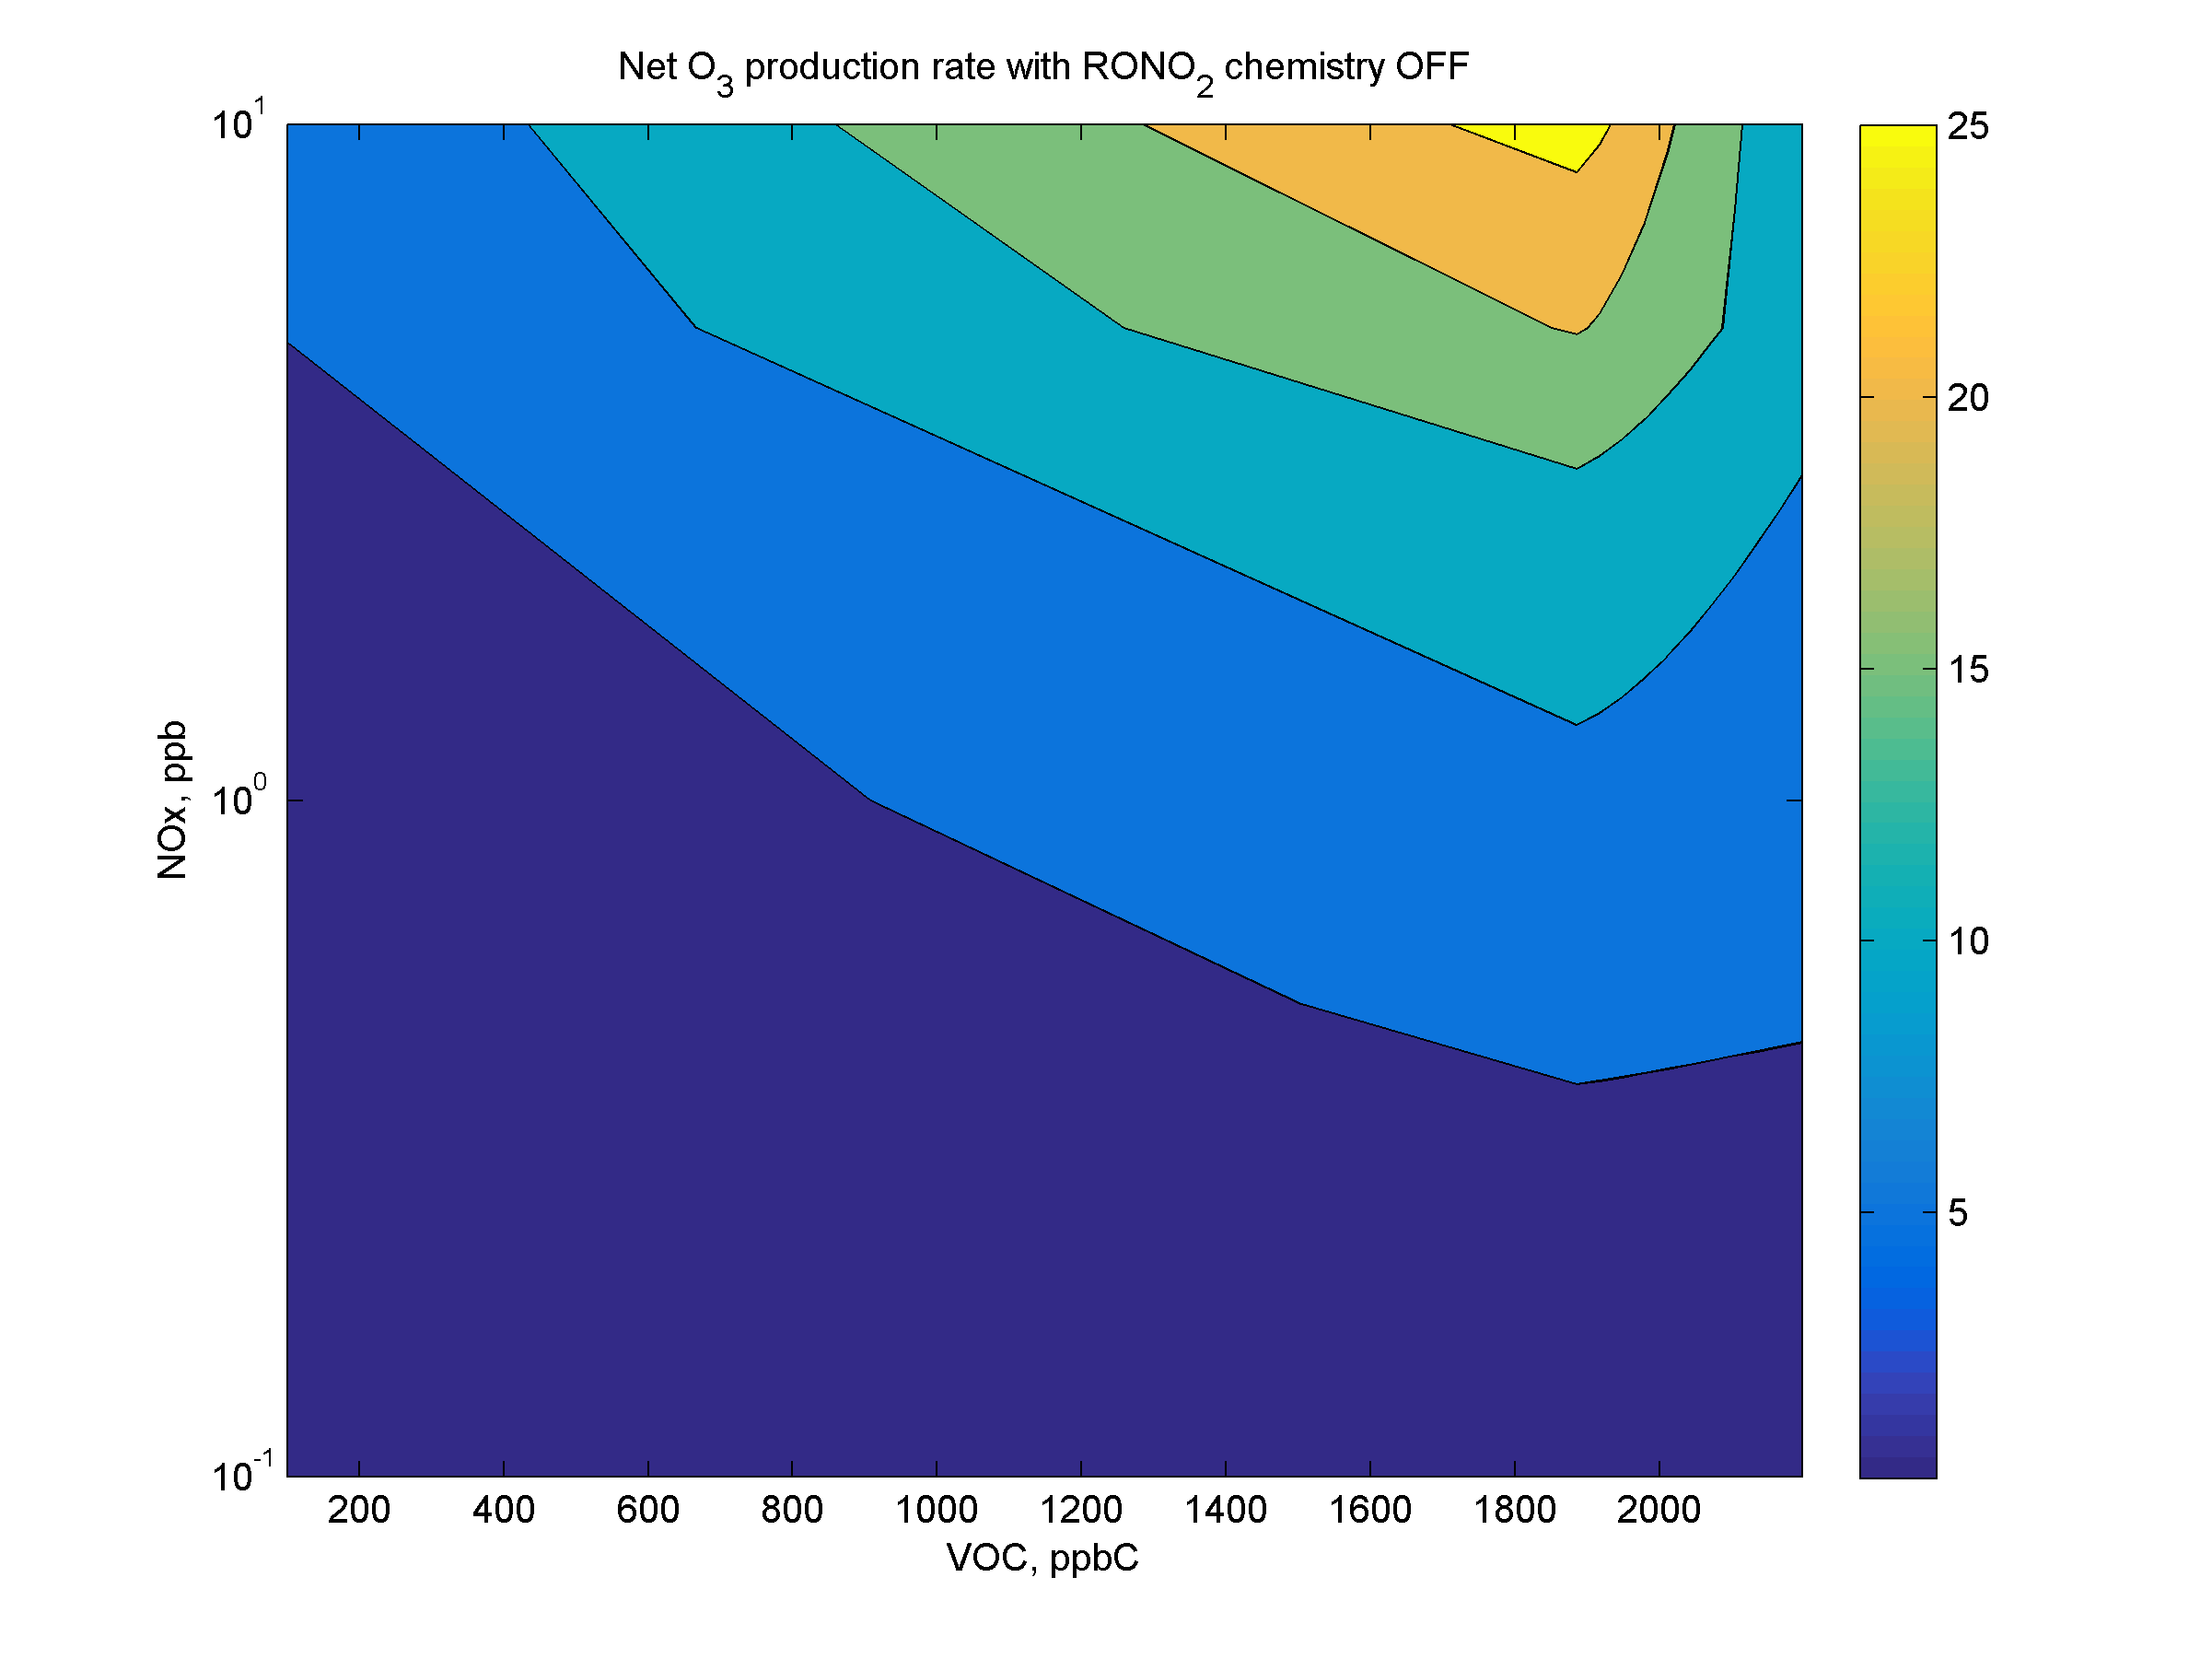
\includegraphics[width=.99\linewidth]{D:/FACSIMILE/ANsCBmodel/matlab/ANsCB_pics/ANsNOxVOC/noAN/chem_noAN_netO3rate_withINORG_NOx_1ppb_100ppb.png}
  \captionof{figure}{Isopleths giving net rate of $O_3$ production (ppb/h, color) as a function of $VOC$ (ppbC) and $NO_x$ (ppb) in the first modelling experiment with alkyl nitrate chemistry switched off combined with an additional run with inorganic chemistry only (i.e. the only $VOC$ is $CO$).}\label{fig:noAN_netO3rate}
\end{minipage}
\end{figure}

Rewrite!

The same kind of plot can be found in Figure \ref{fig:noAN_netO3rate}, which is produced using data from our model from the first experiment with alkyl nitrate chemistry switched off. Taking into account the fact that the maximum $NO_x$ mixing ratio considered in the experiment is 10 ppb, our results are directly comparable only with a part of the data from Figure \ref{fig:Sillman1999}, namely with those inside the green dashed square. Moreover, since the minimum $NO_x$ mixing ratio considered in the experiment is 5 ppt, while the corresponding value in Figure \ref{fig:Sillman1999} is 1 ppb, a negative $O_3$ production rate is seen in our results, whereas it stays out of range of Figure \ref{fig:Sillman1999}.

One can see the same pattern in these two figures. At high $VOC$/$NO_x$ ratios, the rate of $O_3$ production increases with increasing $NO_x$ and reaches its maximum at the highest $NO_x$ and $VOC$ levels (which corresponds to the top right corner of the green dashed square). The change in $O_3$ production rate at high $VOC$/$NO_x$ ratios in our model is largely insensitive to $VOC$, which fits into the theory. At low $VOC$/$NO_x$ ratios the $O_3$ production rate starts to depend on $VOC$ concentration also resembling the behaviour of ozone isopleths at the top left corner of the green dashed square. The overall tendency of $O_3$ production rate to increase with increasing $VOC$ and $NO_x$ is present in both figures showing that the model reproduces this feature according to the theory. However, the modelled values of $O_3$ production rates are much lower than those in Figure \ref{fig:Sillman1999}: in the model the maximum production rate is 9 ppb/h, while in theory it is 30 ppb/h, meaning that our model underestimates the $O_3$ production rate, but reproduces some features of the relationship between $O_3$, $NO_x$ and $VOC$.

\section{Results} \label{sec:res}
\subsection{Sensitivity of $O_3$ production to alkyl nitrate chemistry}

To evaluate the sensitivity of $O_3$ production (efficiency) to alkyl nitrate ($RONO_2$) chemistry under different $NO_x$ and $VOC$ conditions a number of simulations were carried out. In these simulations the chemical mechanism of the model was adjusted to either include or exclude the formation and loss of alkyl nitrates, which was accomplished by switching on and off all reactions that involve $RONO_2$ while keeping the rest of the mechanism unchanged. 

As it has been noted in Section \ref{sec:intro}, the relationship between $O_3$ and $RONO_2$ production rates is controlled by the branching ratio ($\alpha_3$) between reactions:
\begin{equation}\label{reac:RO2+NO=RO+NO2}
RO_2 + NO \xrightarrow{1-\alpha_3} RO + NO_2
\end{equation}
\begin{equation}\label{reac:RO2+NO=RONO2}
RO_2 + NO \xrightarrow{\alpha_3} RONO_2
\end{equation}
Reaction (\ref{reac:RO2+NO=RO+NO2}) leads to $O_3$ production and $NO$ regeneration, resulting in continuing $O_3$ production, while reaction (\ref{reac:RO2+NO=RONO2}) terminates this process. Branching ratios used in the model are taken from the MCM v3.3, and their values (Table \ref{tab:ANbranching}) were kept constant in all model runs.

\begin{table} %  AN branching ratios
\caption{Branching ratios for the formation of alkyl nitrates from their precursor peroxy radicals and $NO$ (taken from the MCM v3.3 (2015)).}\label{tab:ANbranching}
\centering
\begin{tabular}{cc}
\hline
Alkyl nitrate    & Branching ratio \\
\hline
methyl           & 0.001 \\
ethyl            & 0.009 \\
iso-propyl       & 0.042 \\
n-propyl         & 0.020 \\
n-butyl          & 0.033 \\
sec-butyl        & 0.090 \\
iso-butyl        & 0.033 \\ 
tert-butyl       & 0.025 \\
n-pentyl         & 0.052 \\
2-pentyl         & 0.129 \\
3-pentyl         & 0.131 \\
2-methylbutyl    & 0.052 \\
3-methyl-2-butyl & 0.141 \\
2-methyl-2-butyl & 0.047 \\
\hline
\end{tabular}
\end{table}

Figure \ref{fig:netO3rate_noAN_withAN_diff} shows isopleths of net $O_3$ production rate as a function of $NO_x$ and sum of $VOCs$ initial concentrations from two series of model runs (with and without alkyl chemistry) and the difference between them. Since the actual formation of $O_3$ in our model starts at 250 ppt of $NO_x$, Figure \ref{fig:netO3rate_noAN_withAN_diff} summarises modelling data from experiments with $NO_x$ initial mixing ratios from 250 ppt till 100 ppb.

\begin{figure} % netO3rate noAN withAN diff
\centering
\begin{minipage}{.3\textwidth}
  \centering
  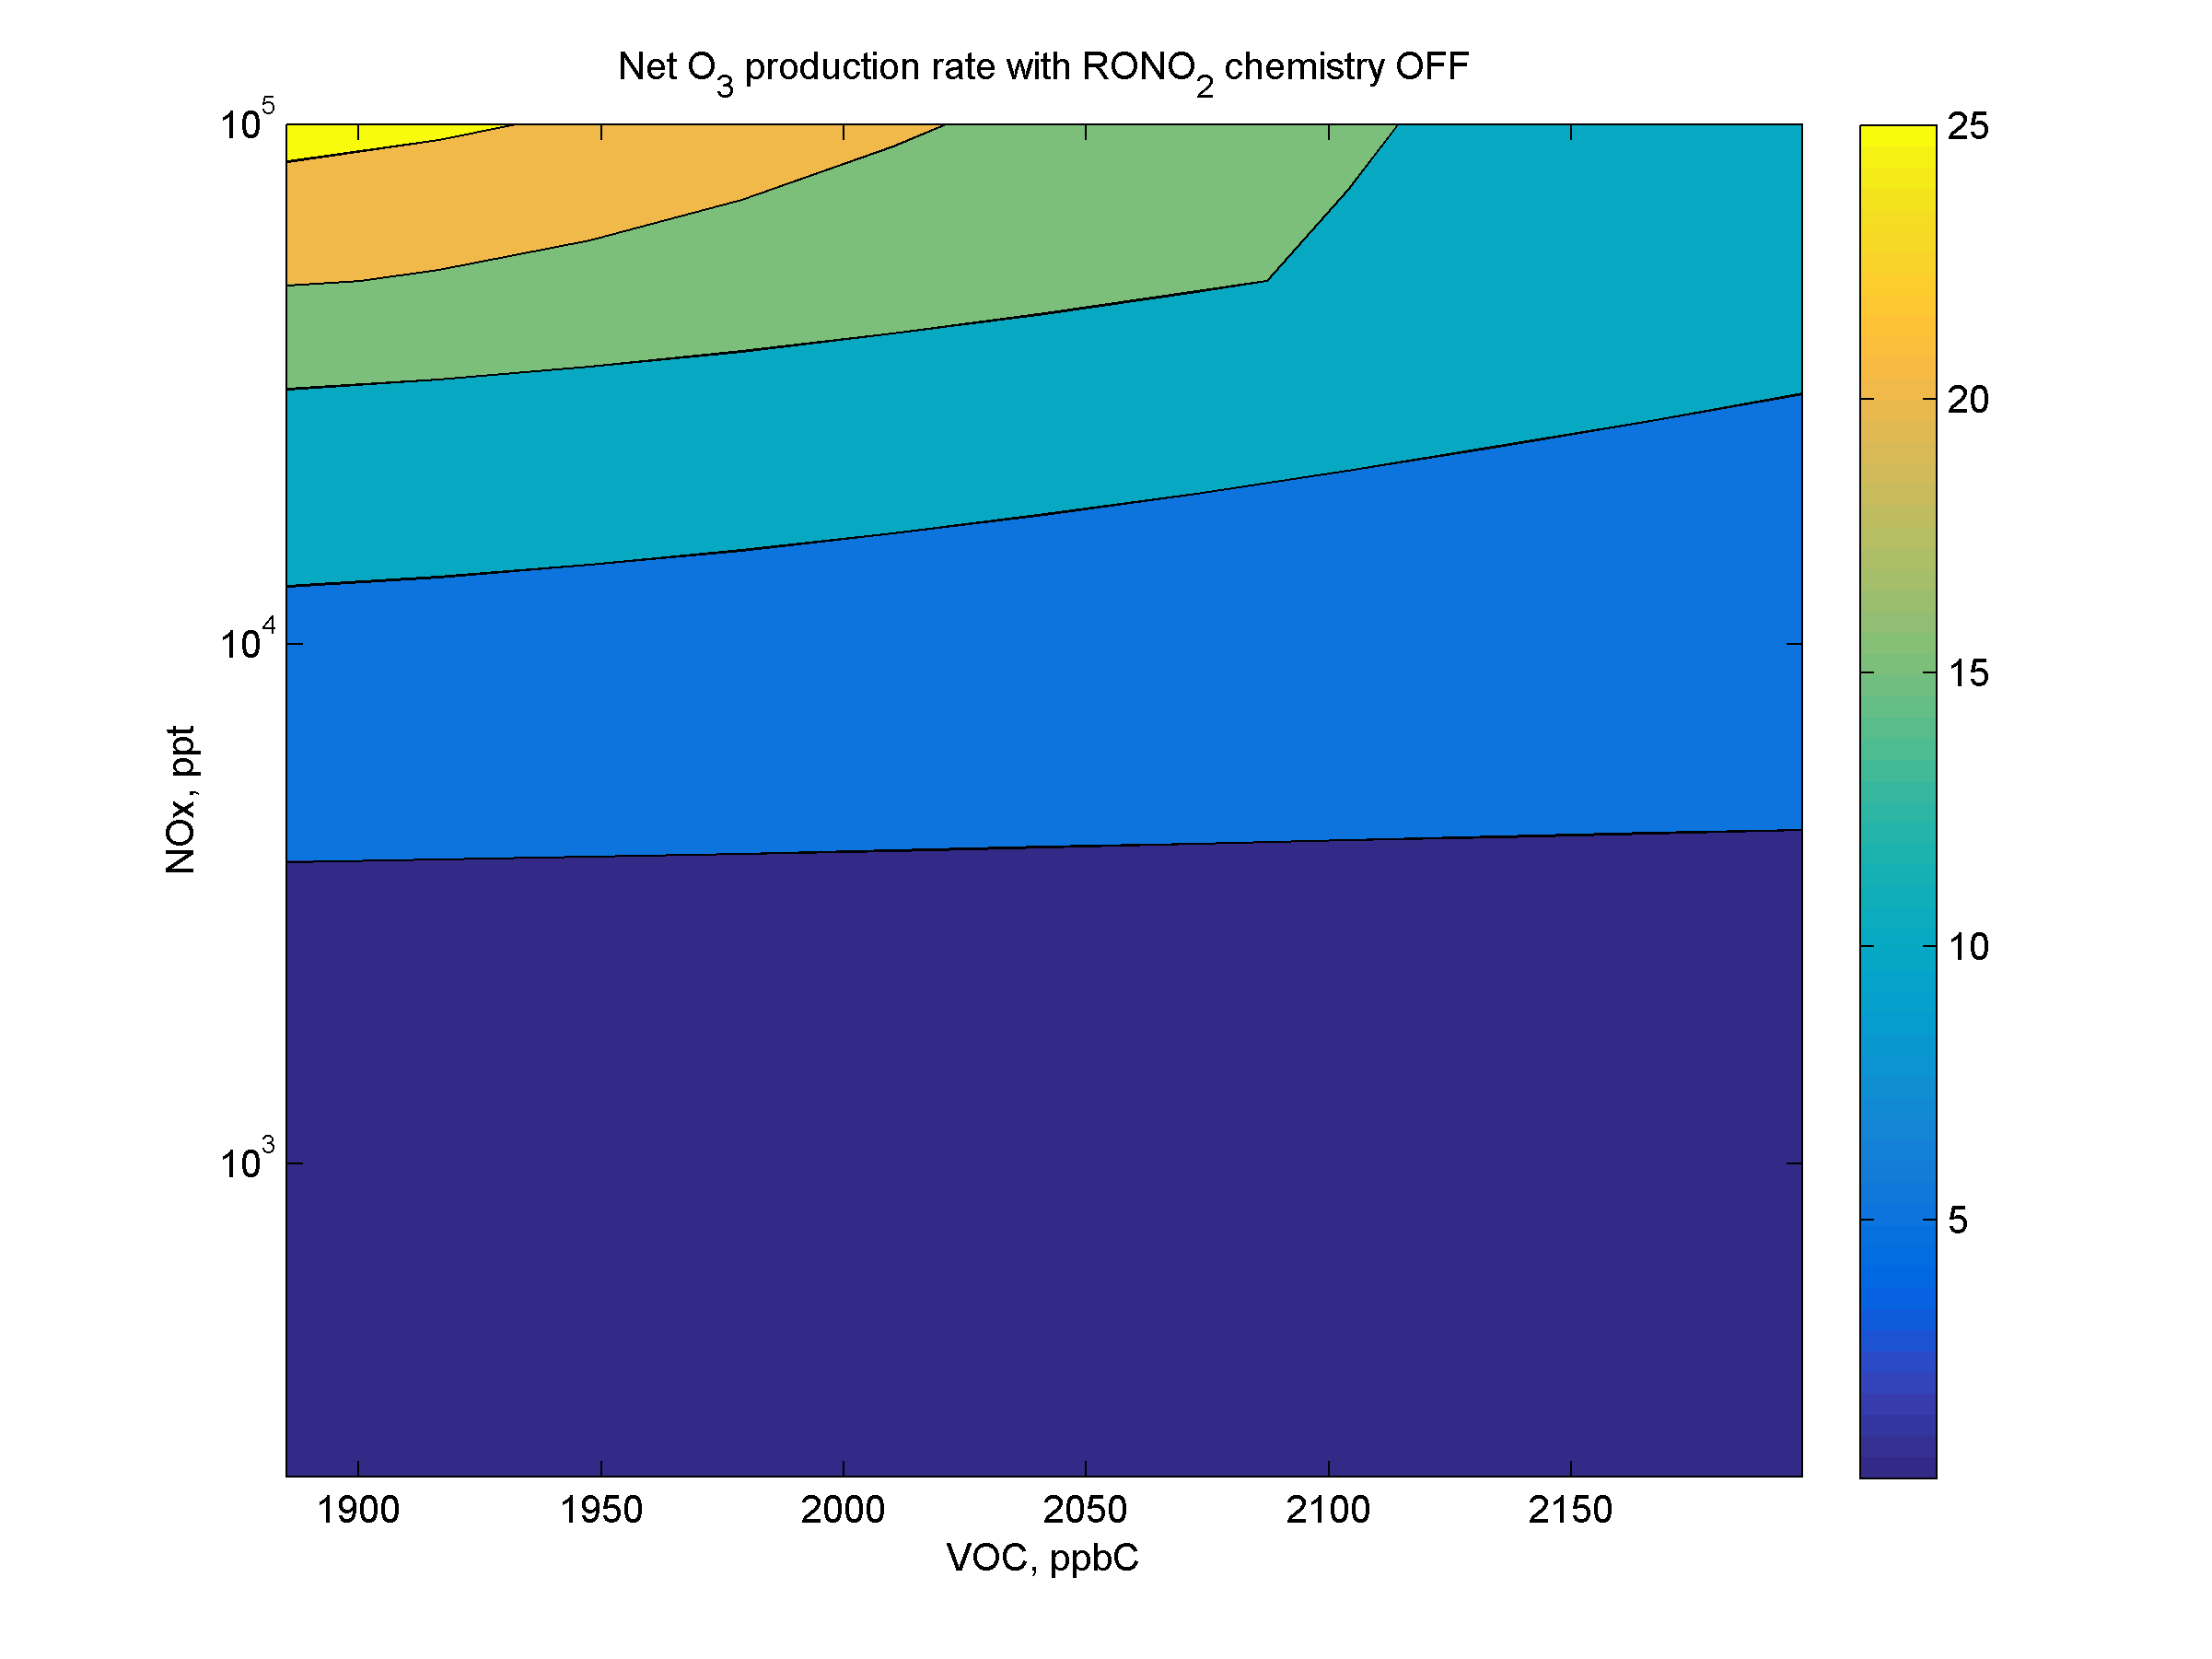
\includegraphics[width=.99\linewidth]{D:/FACSIMILE/ANsCBmodel/matlab/ANsCB_pics/ANsNOxVOC/noAN/chem_noAN_netO3rate_noINORG_NOx_250ppt_100ppb.png}
\end{minipage}
\begin{minipage}{.3\textwidth}
  \centering
  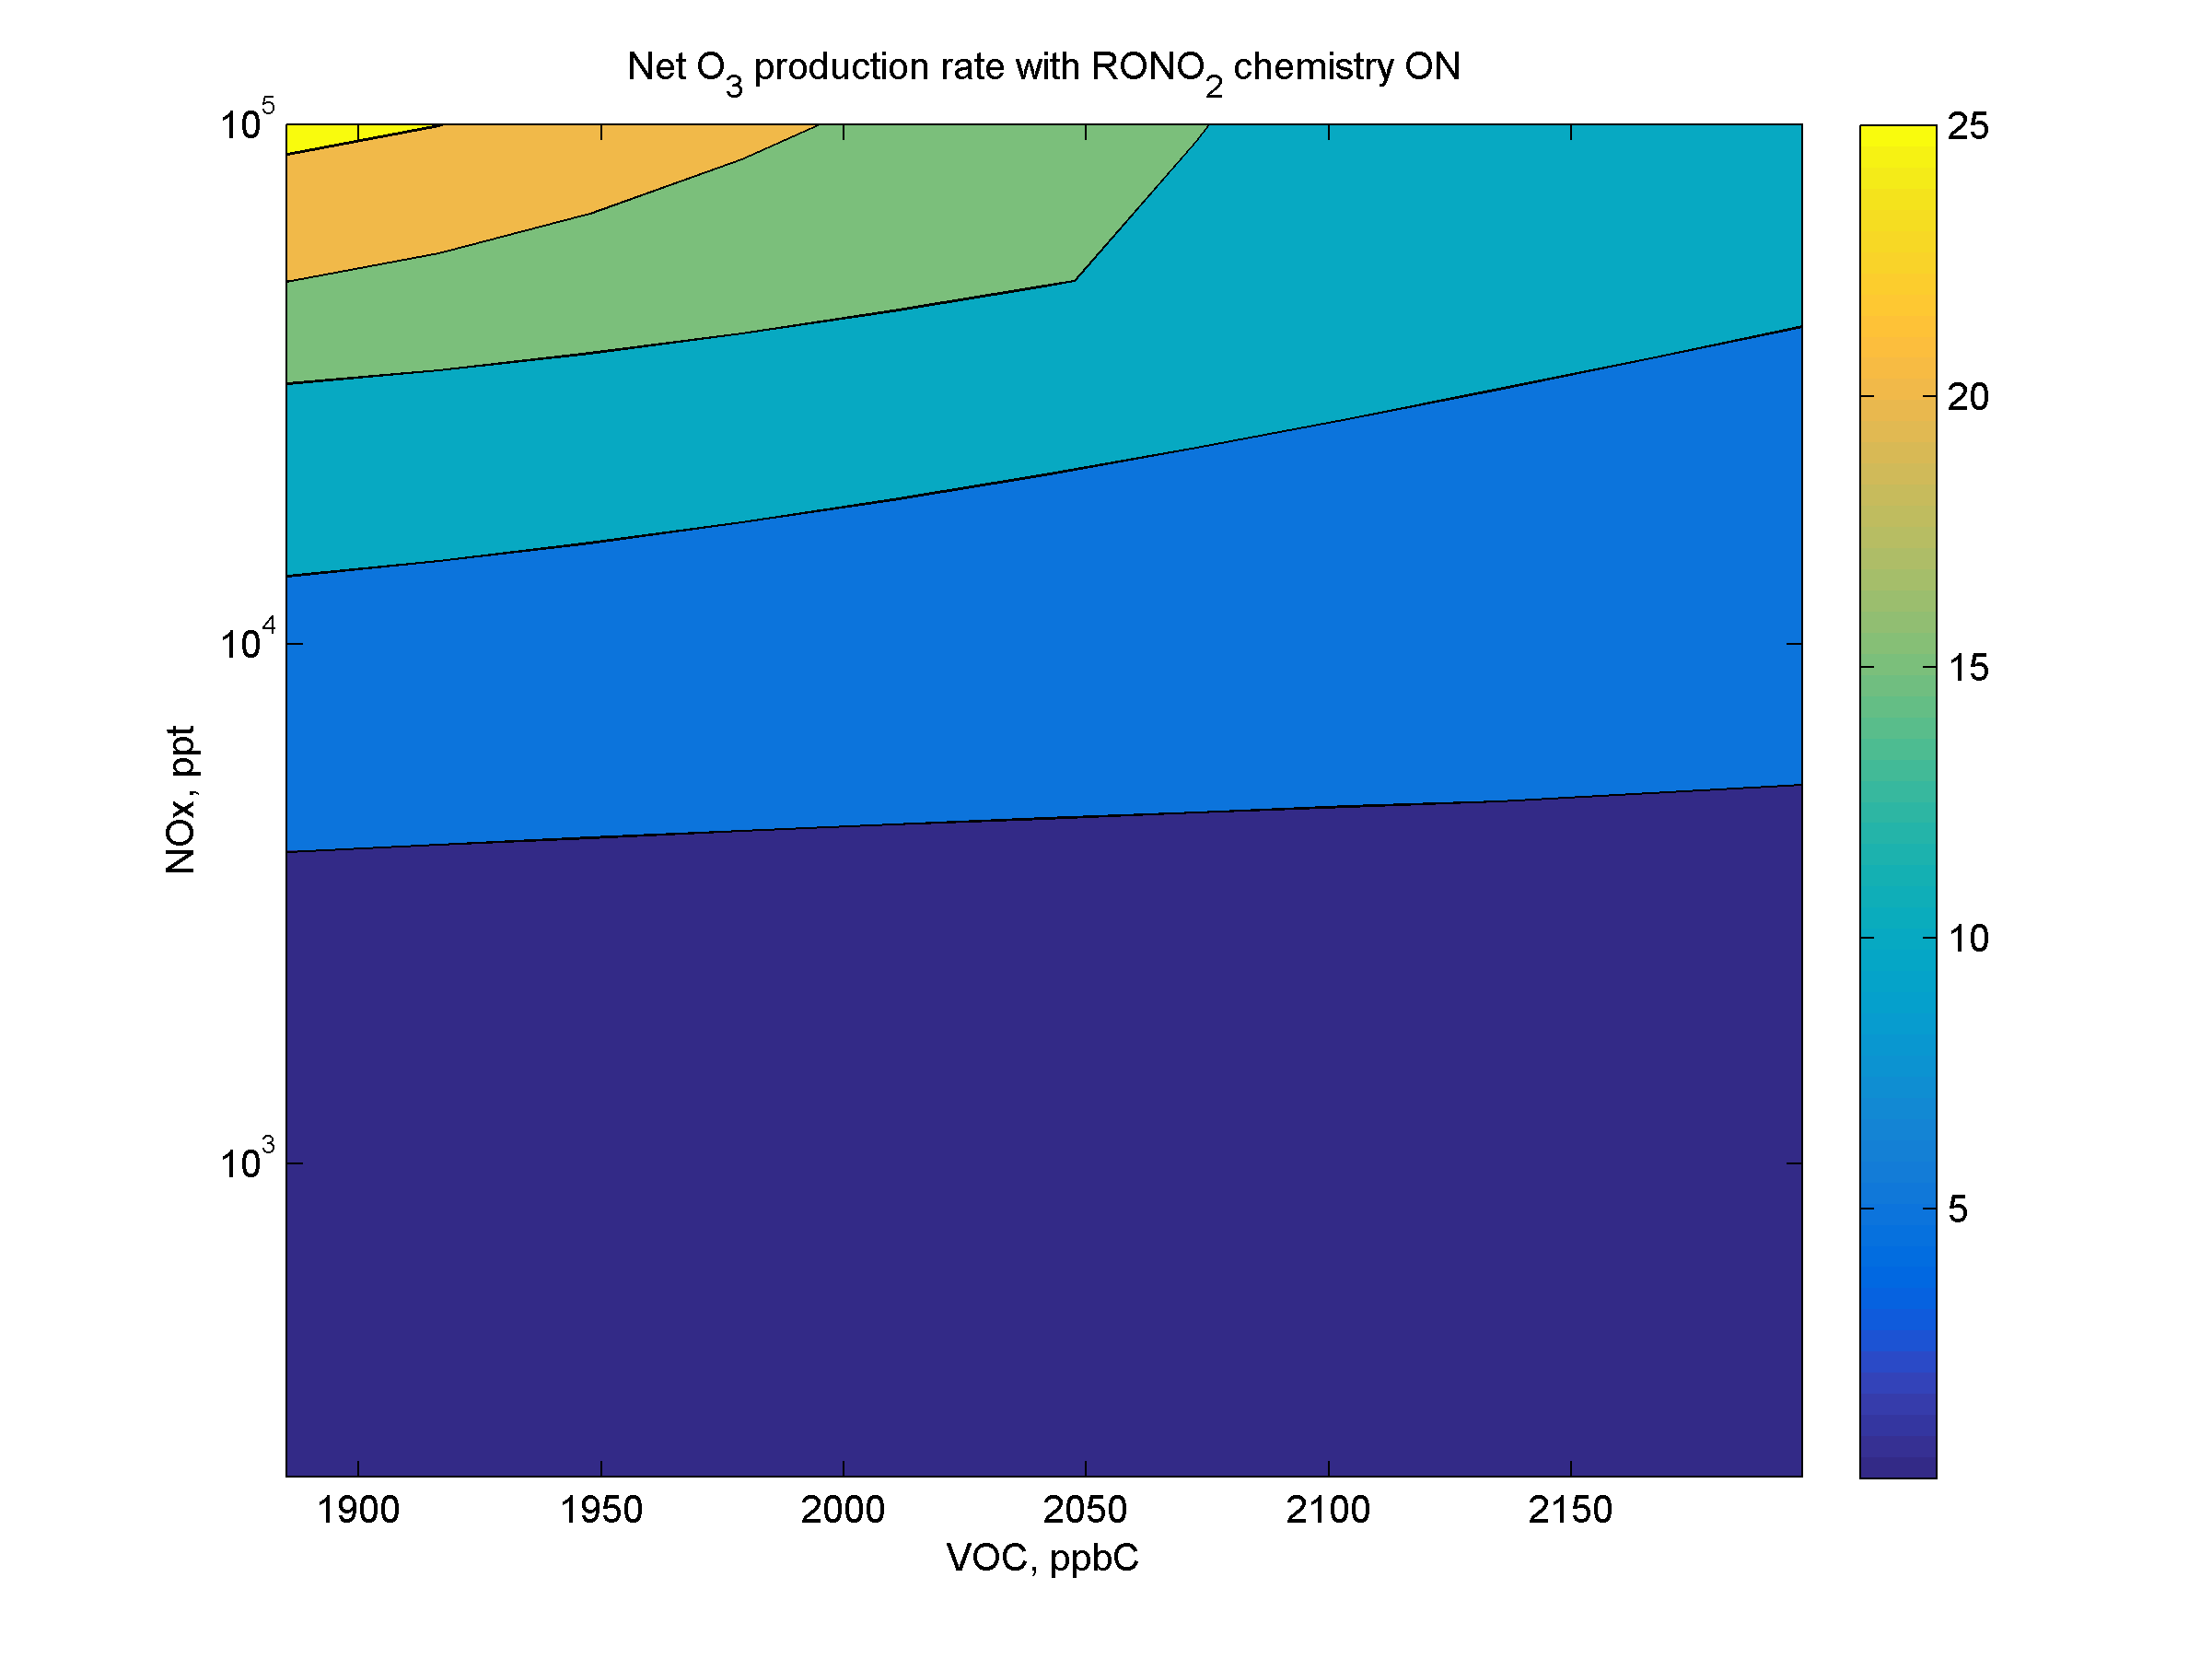
\includegraphics[width=.99\linewidth]{D:/FACSIMILE/ANsCBmodel/matlab/ANsCB_pics/ANsNOxVOC/allAN/chem_allAN_netO3rate_noINORG_NOx_250ppt_100ppb.png}
\end{minipage}
\begin{minipage}{.3\textwidth}
  \centering
  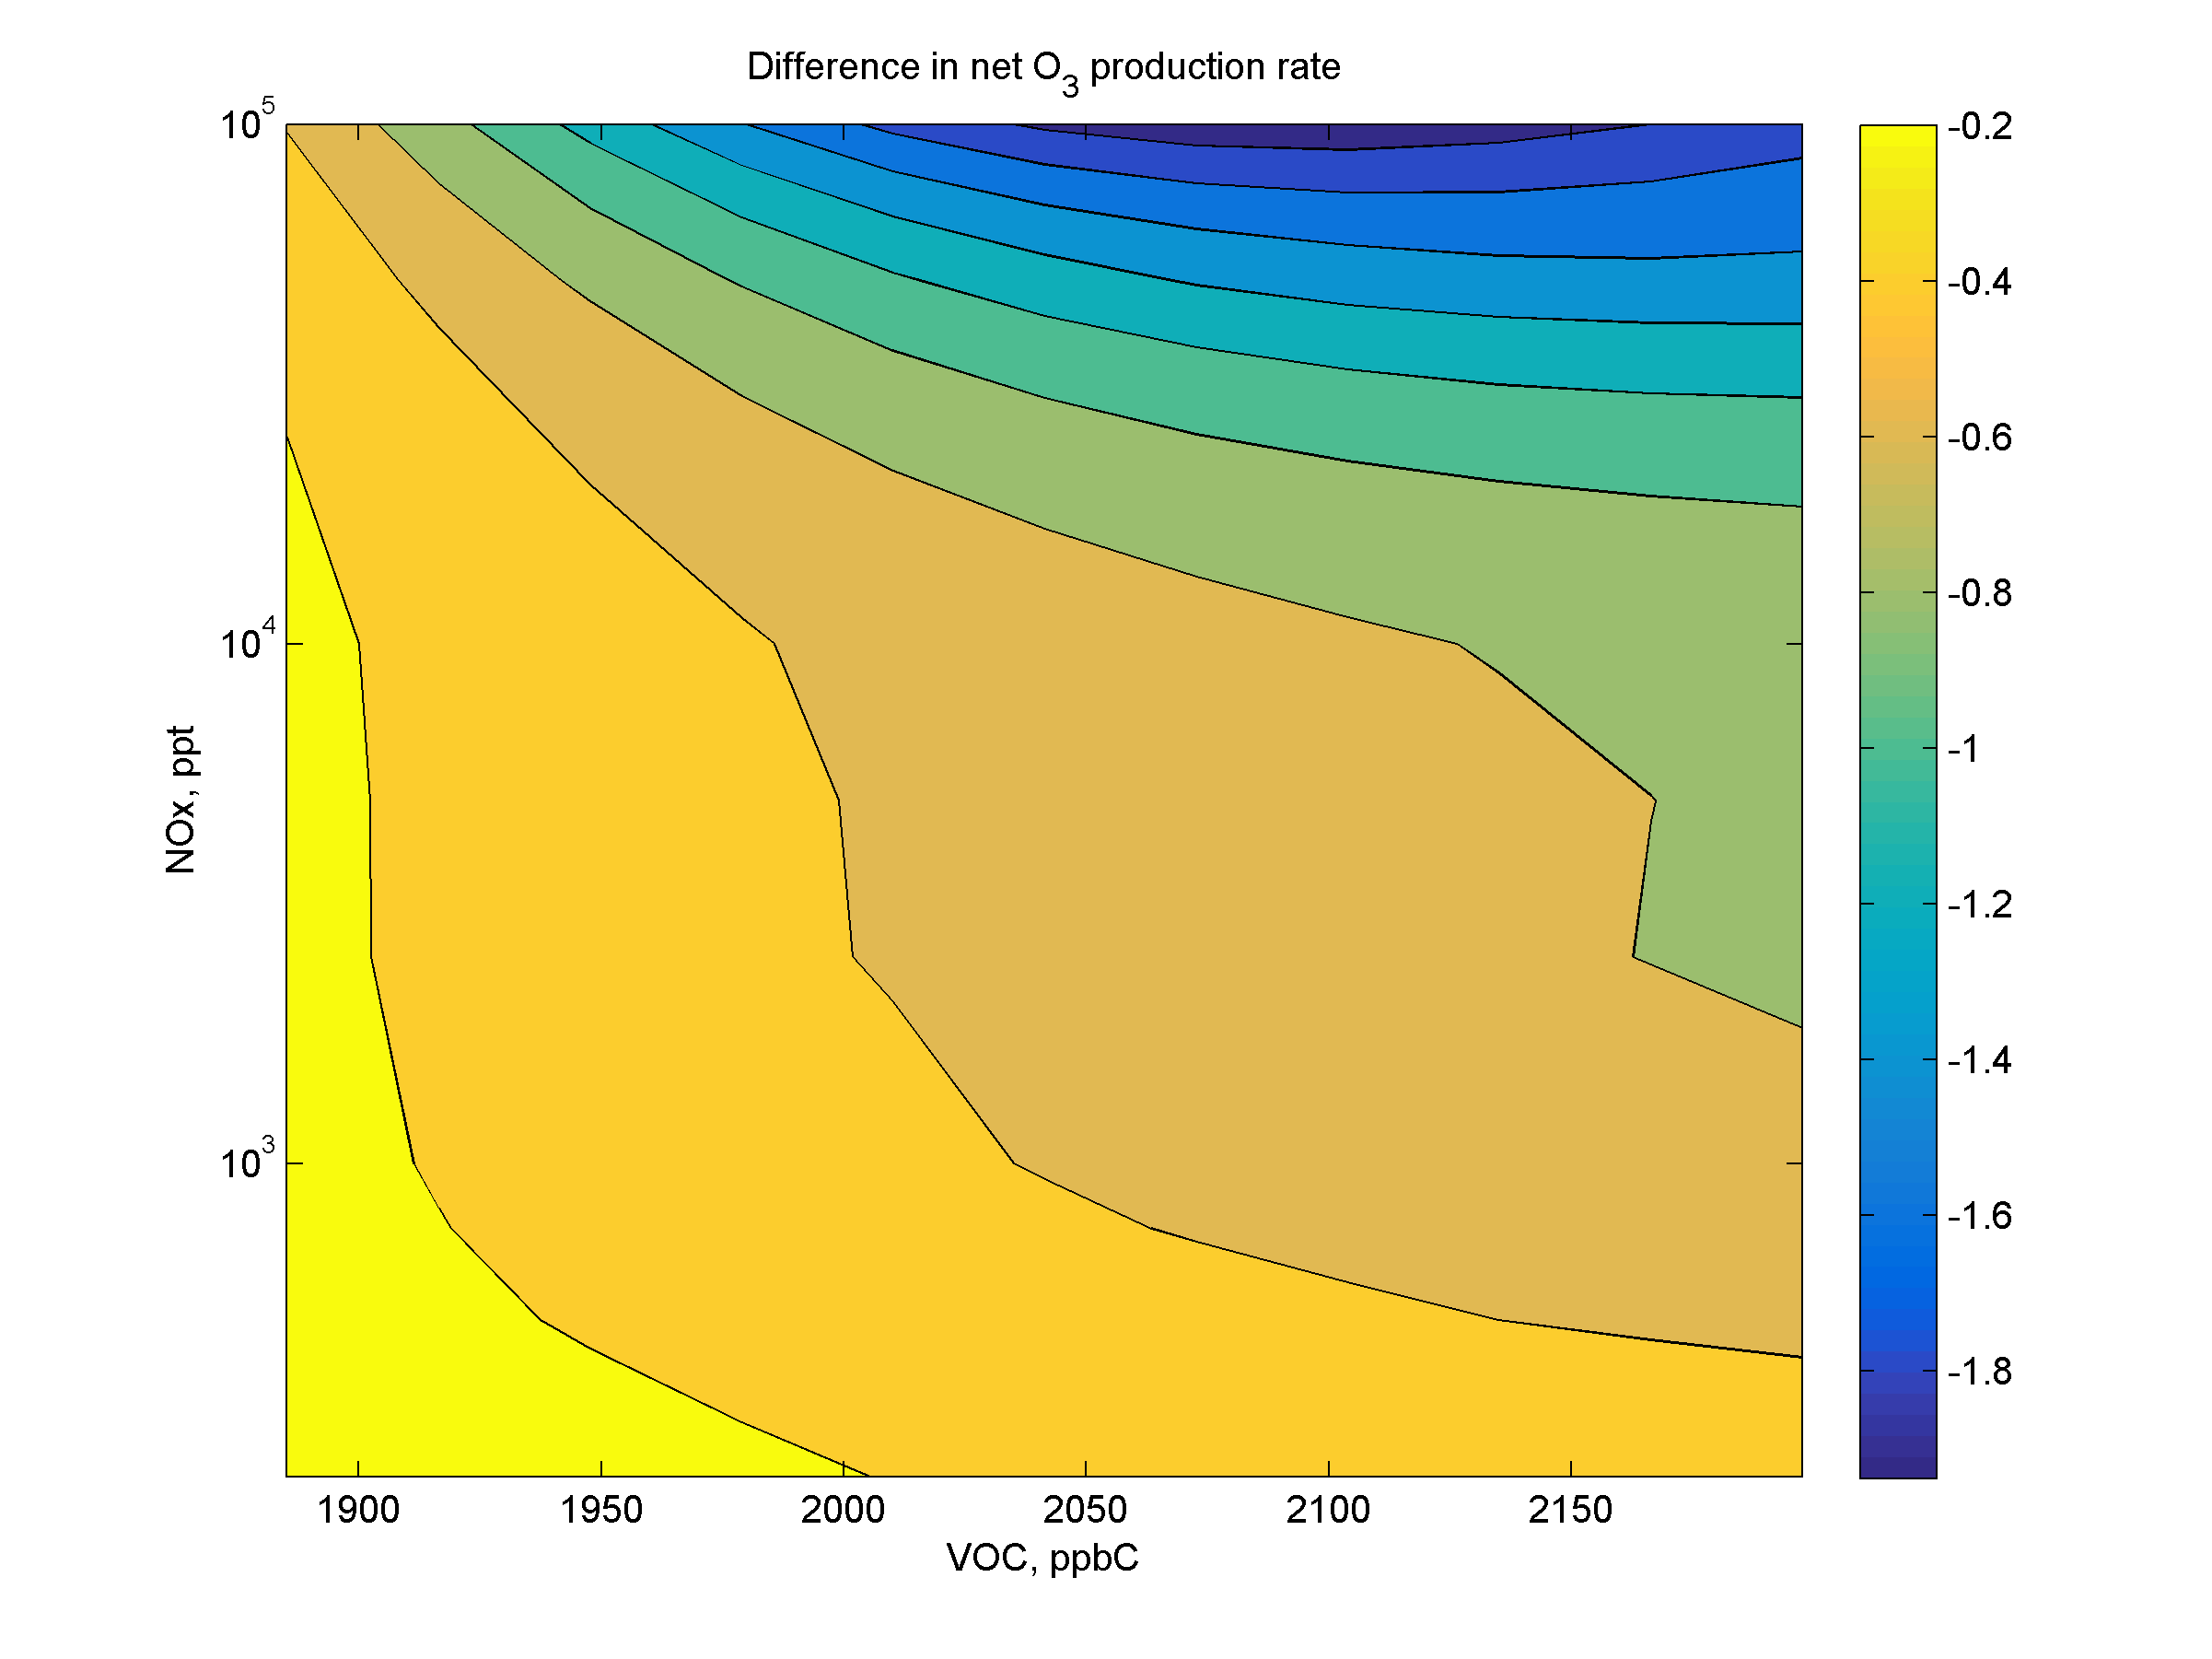
\includegraphics[width=.99\linewidth]{D:/FACSIMILE/ANsCBmodel/matlab/ANsCB_pics/ANsNOxVOC/allAN/chem_allAN_netO3ratediff_noINORG_NOx_250ppt_100ppb.png}
\end{minipage}
\caption{Isopleths giving net rate of $O_3$ production (ppb/h, color) as a function of $VOC$ (ppbC) and $NO_x$ (ppb) with alkyl nitrate chemistry switched off (left) and switched on (middle). Difference between them is shown on the right.}\label{fig:netO3rate_noAN_withAN_diff}
\end{figure}

As expected, the inclusion of alkyl nitrate chemistry slows down the net $O_3$ production rate. At low $NO_x$ and $VOCs$ initial levels, this slowdown is -0.2...-0.6 ppb of $O_3$ per hour. As $NO_x$ and $VOCs$ levels increase the $O_3$ production rate decreases, reaching the maximum decrease of -1.94 ppb of $O_3$ per hour at 100 ppb of $NO_x$ and $VOCs$ level from case I (not the highest $VOCs$ level). At the range of $NO_x$ levels from 1 ppb to 10 ppb the $O_3$ production rate is slightly more sensitive to $VOCs$ levels, while it is almost insensitive to $VOCs$ at $NO_x$ levels higher than 10 ppb and 2050 ppbC of $VOCs$. 

\begin{figure} % netO3mixrat noAN withAN diff
\centering
\begin{minipage}{.3\textwidth}
  \centering
  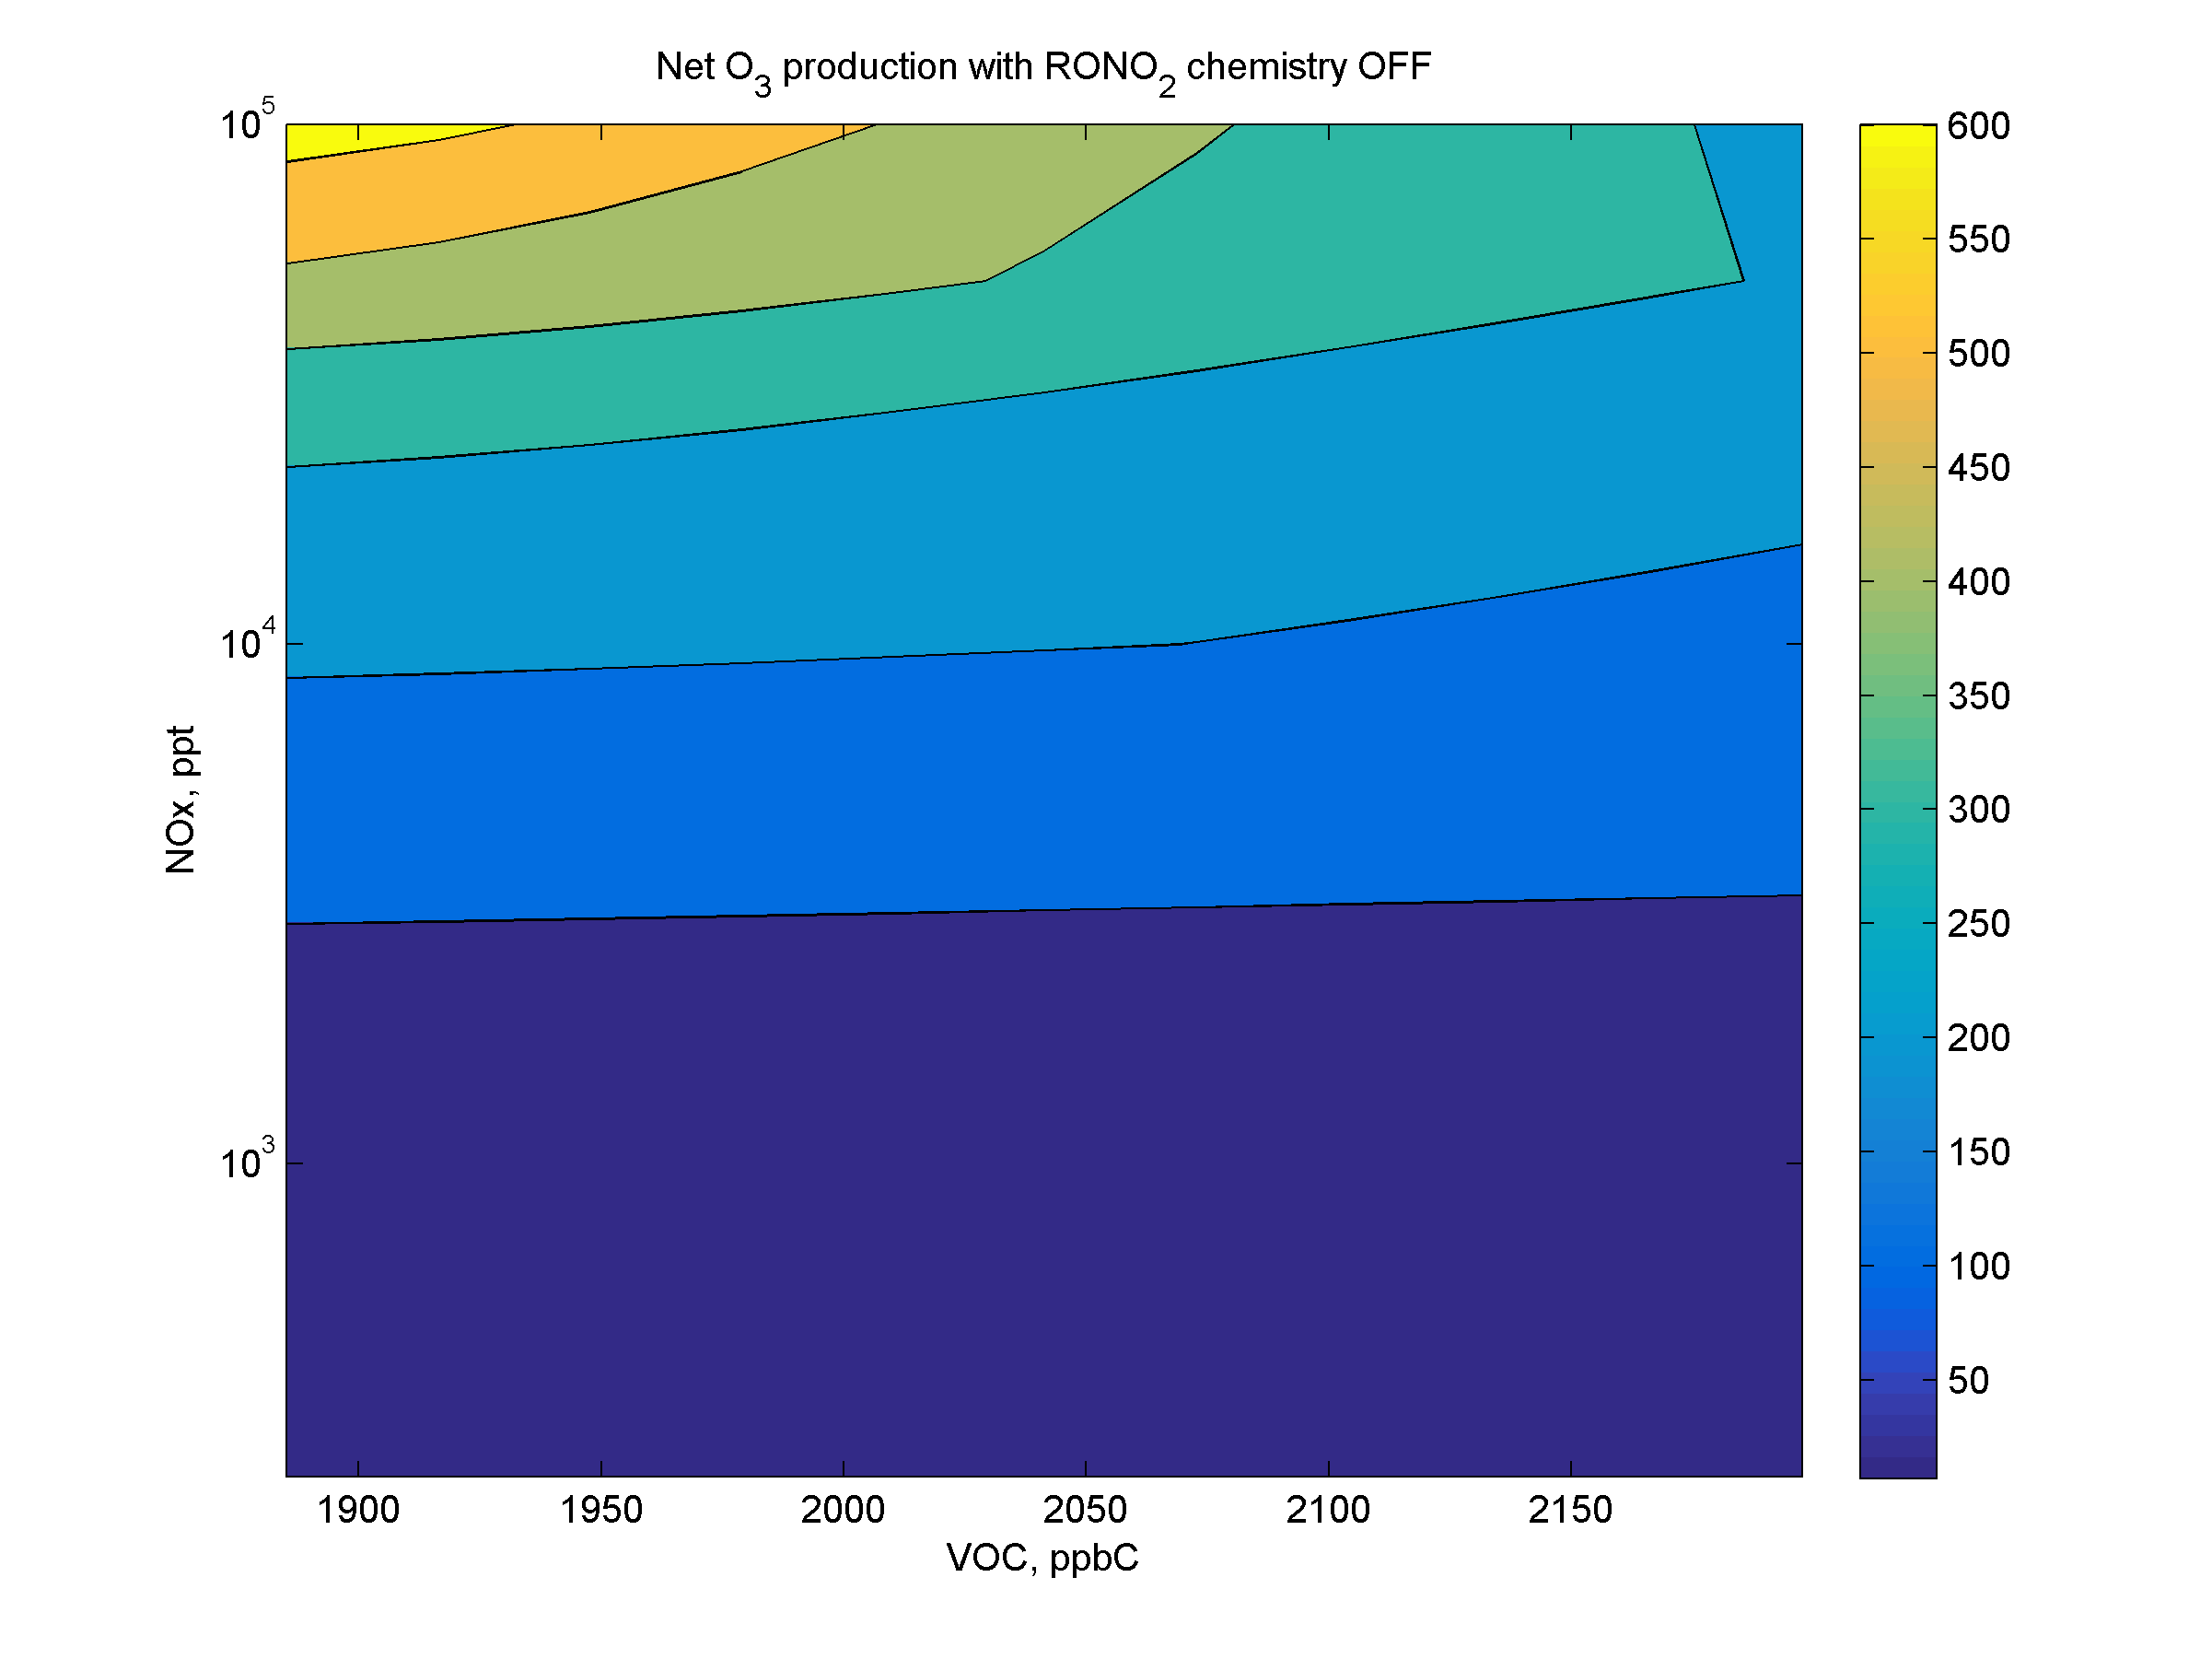
\includegraphics[width=.99\linewidth]{D:/FACSIMILE/ANsCBmodel/matlab/ANsCB_pics/ANsNOxVOC/noAN/chem_noAN_netO3mixrat_noINORG_NOx_250ppt_100ppb.png}
\end{minipage}
\begin{minipage}{.3\textwidth}
  \centering
  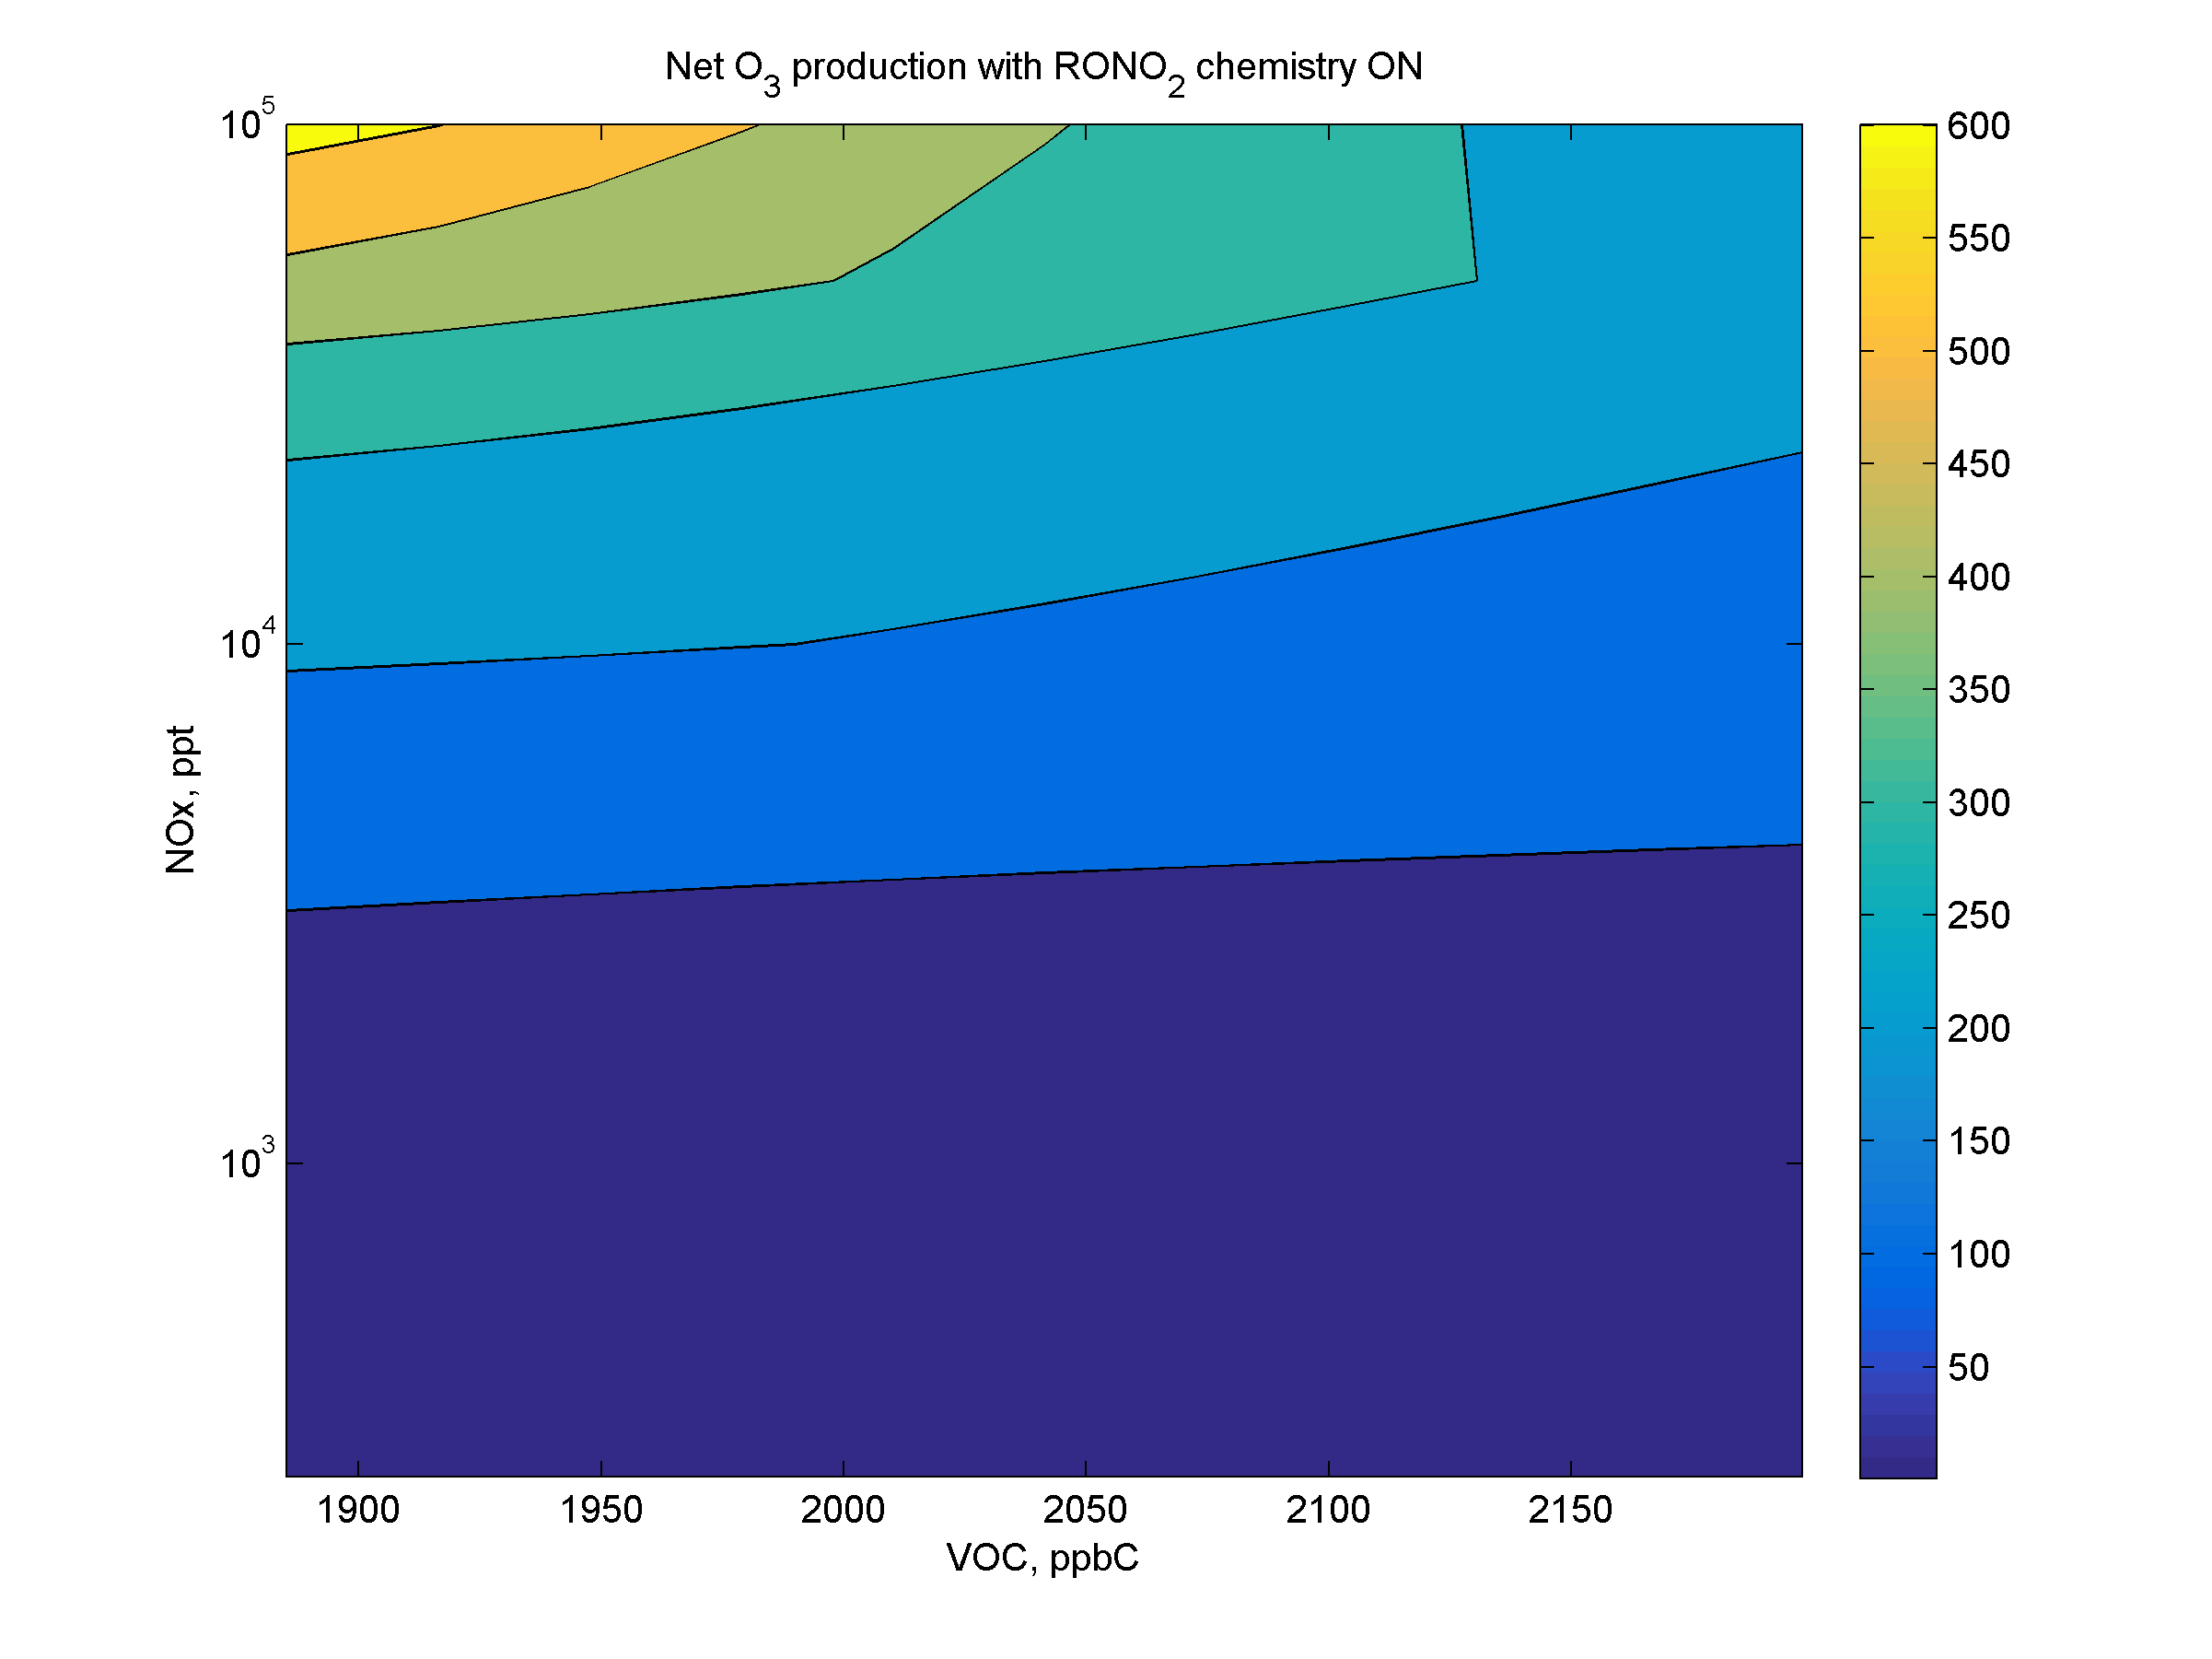
\includegraphics[width=.99\linewidth]{D:/FACSIMILE/ANsCBmodel/matlab/ANsCB_pics/ANsNOxVOC/allAN/chem_allAN_netO3mixrat_noINORG_NOx_250ppt_100ppb.png}
\end{minipage}
\begin{minipage}{.3\textwidth}
  \centering
  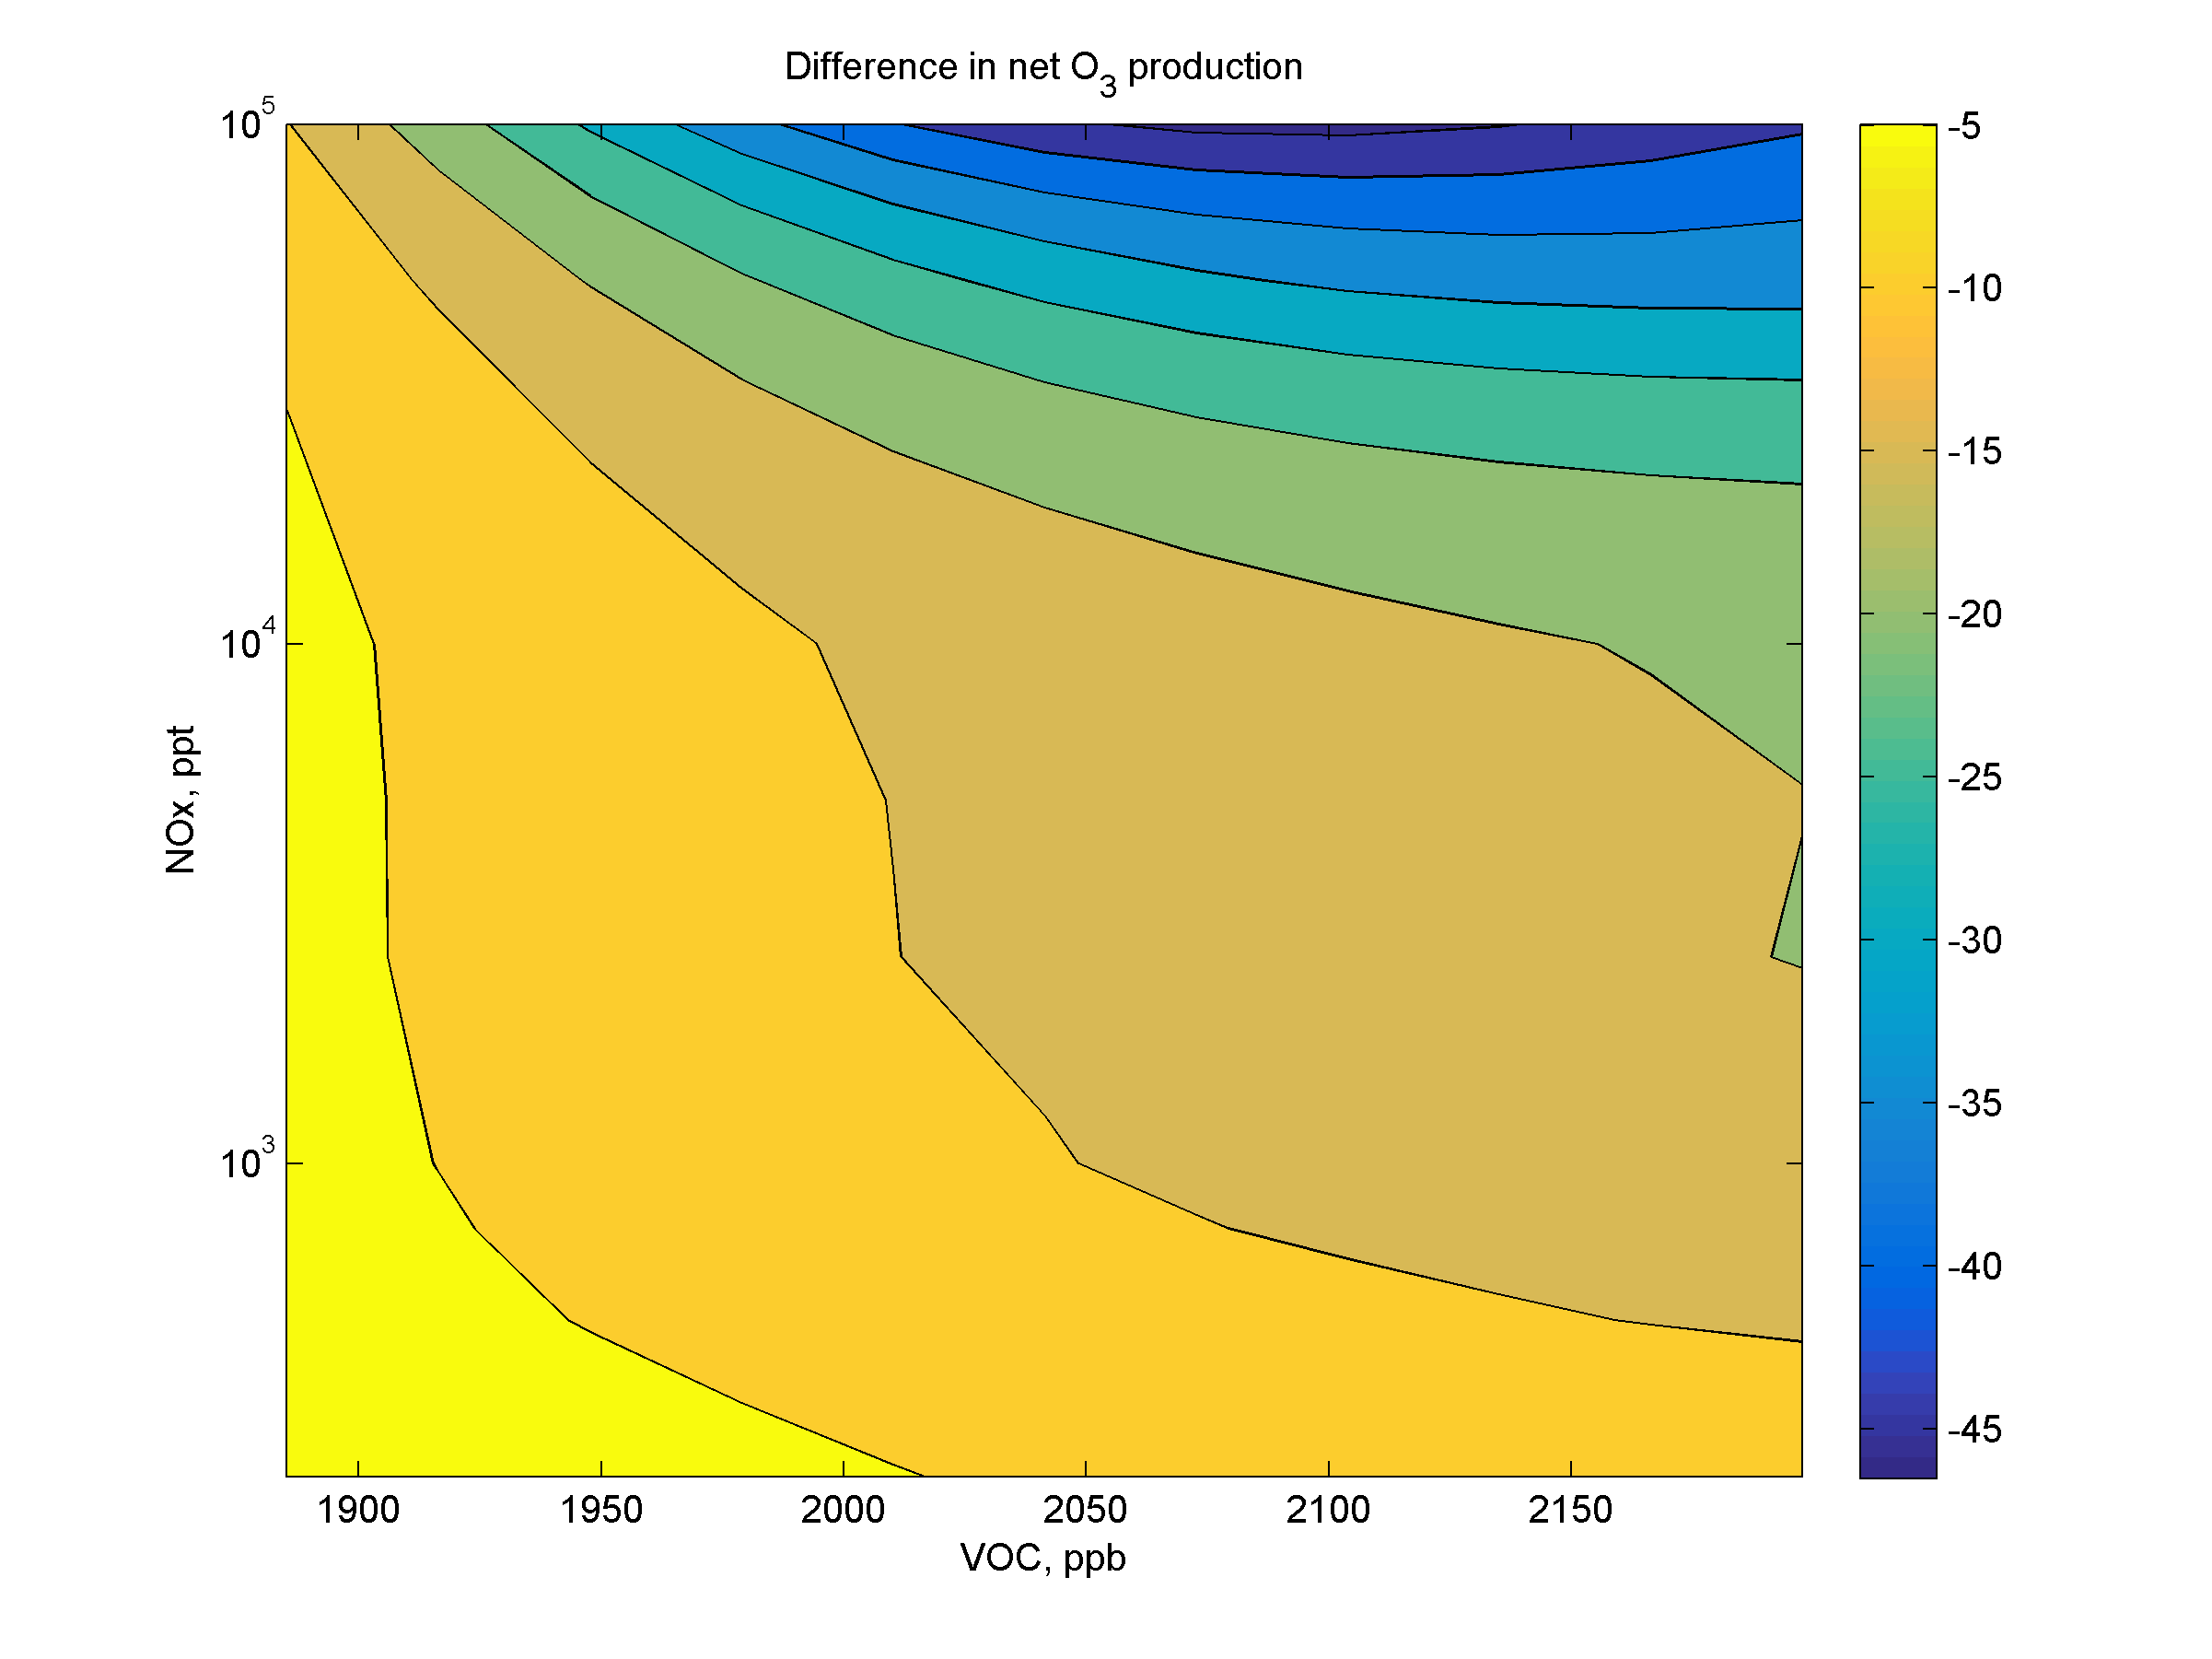
\includegraphics[width=.99\linewidth]{D:/FACSIMILE/ANsCBmodel/matlab/ANsCB_pics/ANsNOxVOC/allAN/chem_allAN_netO3mixratdiff_noINORG_NOx_250ppt_100ppb.png}
\end{minipage}
\caption{Isopleths giving net $O_3$ production (ppb, color) as a function of $VOC$ (ppbC) and $NO_x$ (ppb) with alkyl nitrate chemistry switched off (left) and switched on (middle). Difference between them is shown on the right. Net production = final - initial value of $O_3$ mixing ratio.}\label{fig:netO3mixrat_noAN_withAN_diff}
\end{figure}

The change in net rate of $O_3$ production due to inclusion of alkyl nitrate chemistry into the chemical mechanism has a direct impact on absolute $O_3$ levels calculated by the model. Figure \ref{fig:netO3mixrat_noAN_withAN_diff} shows that the net $O_3$ production (difference between final and initial $O_3$ mixing ratio) is smaller when alkyl nitrate chemistry is switched on. At low $NO_x$ and $VOCs$ levels the (negative) change in the net $O_3$ production is 5-10 ppb, at high $NO_x$ and $VOCs$ levels it is 35-45 ppb (per 24 hours) with maximum value of 46.5 ppb. However, these changes in the net $O_3$ production should be treated with care, because the model due to reasons described in Section \ref{sec:method} gives unrealistically high $O_3$ mixing ratios (maximum 650 ppb while typical maximum urban $O_3$ mixing ratio (Los Angeles, Mexico City) is 490 ppb (http://www-personal.umich.edu/~sillman/ozone.htm). Therefore, in this case a more useful estimate of effect of these changes is to express them in percentage form (i.e., compare like with like), and it appears that these changes are very small: ??? respectively.

To see what caused these changes it is useful to look at the net production of the sum of the alkyl nitrates themselves as a function of $NO_x$ and $VOCs$ levels (Figure \ref{fig:endtotalANs}). Since alkyl nitrates are the only sink for $NO_x$ in our model the high production of these species in total was expected. The range is ppb.
However, real concentrations reported from observational studies are of different order, tens of ppt.
\citep{Reeves2007} 10 ppt (ITOP) \citep{Roberts1998} 14 ppt

\citep{Reeves2007}
[In the 'marine' air masses methyl nitrate shows a slightly higher mean concentration to 'other' air masses (2.40 compared to 2.29 ppt), but the concentrations of the other alkyl
nitrates are lower by around 30–50% with the exception of
ethyl nitrate which is lower by about 15% (1.33 compared to
1.57 ppt), such that it becomes the second most abundant alkyl
nitrate.
The highest alkyl
nitrate concentration was observed during flight B031 (air
from New York) for 2-methyl-3-butyl nitrate (13.7 ppt),
when the maximum concentration of 2 + 3-pentyl nitrate
(9.0 ppt) was also measured. It is quite possible that some of
the ‘‘marine’’ maximum concentrations of the alkyl nitrates
were impacted by terrestrial emissions (e.g., 5.4 pptv of
2-methyl-3-butyl nitrate and 1.7 pptv for 2 + 3-pentyl nitrate
observed during flight B030).

The mean NO concentration observed during ITOP (20 plus minus 31 pptv (Lewis et al., 2007)) is below the limit of 100–200 pptv at which the efficiency of the alkyl nitrate formation is reduced because of competition between the reaction of ROO with NO and ROO self/cross reactions (Roberts et al., 1998)]

\begin{figure} % endtotalANs
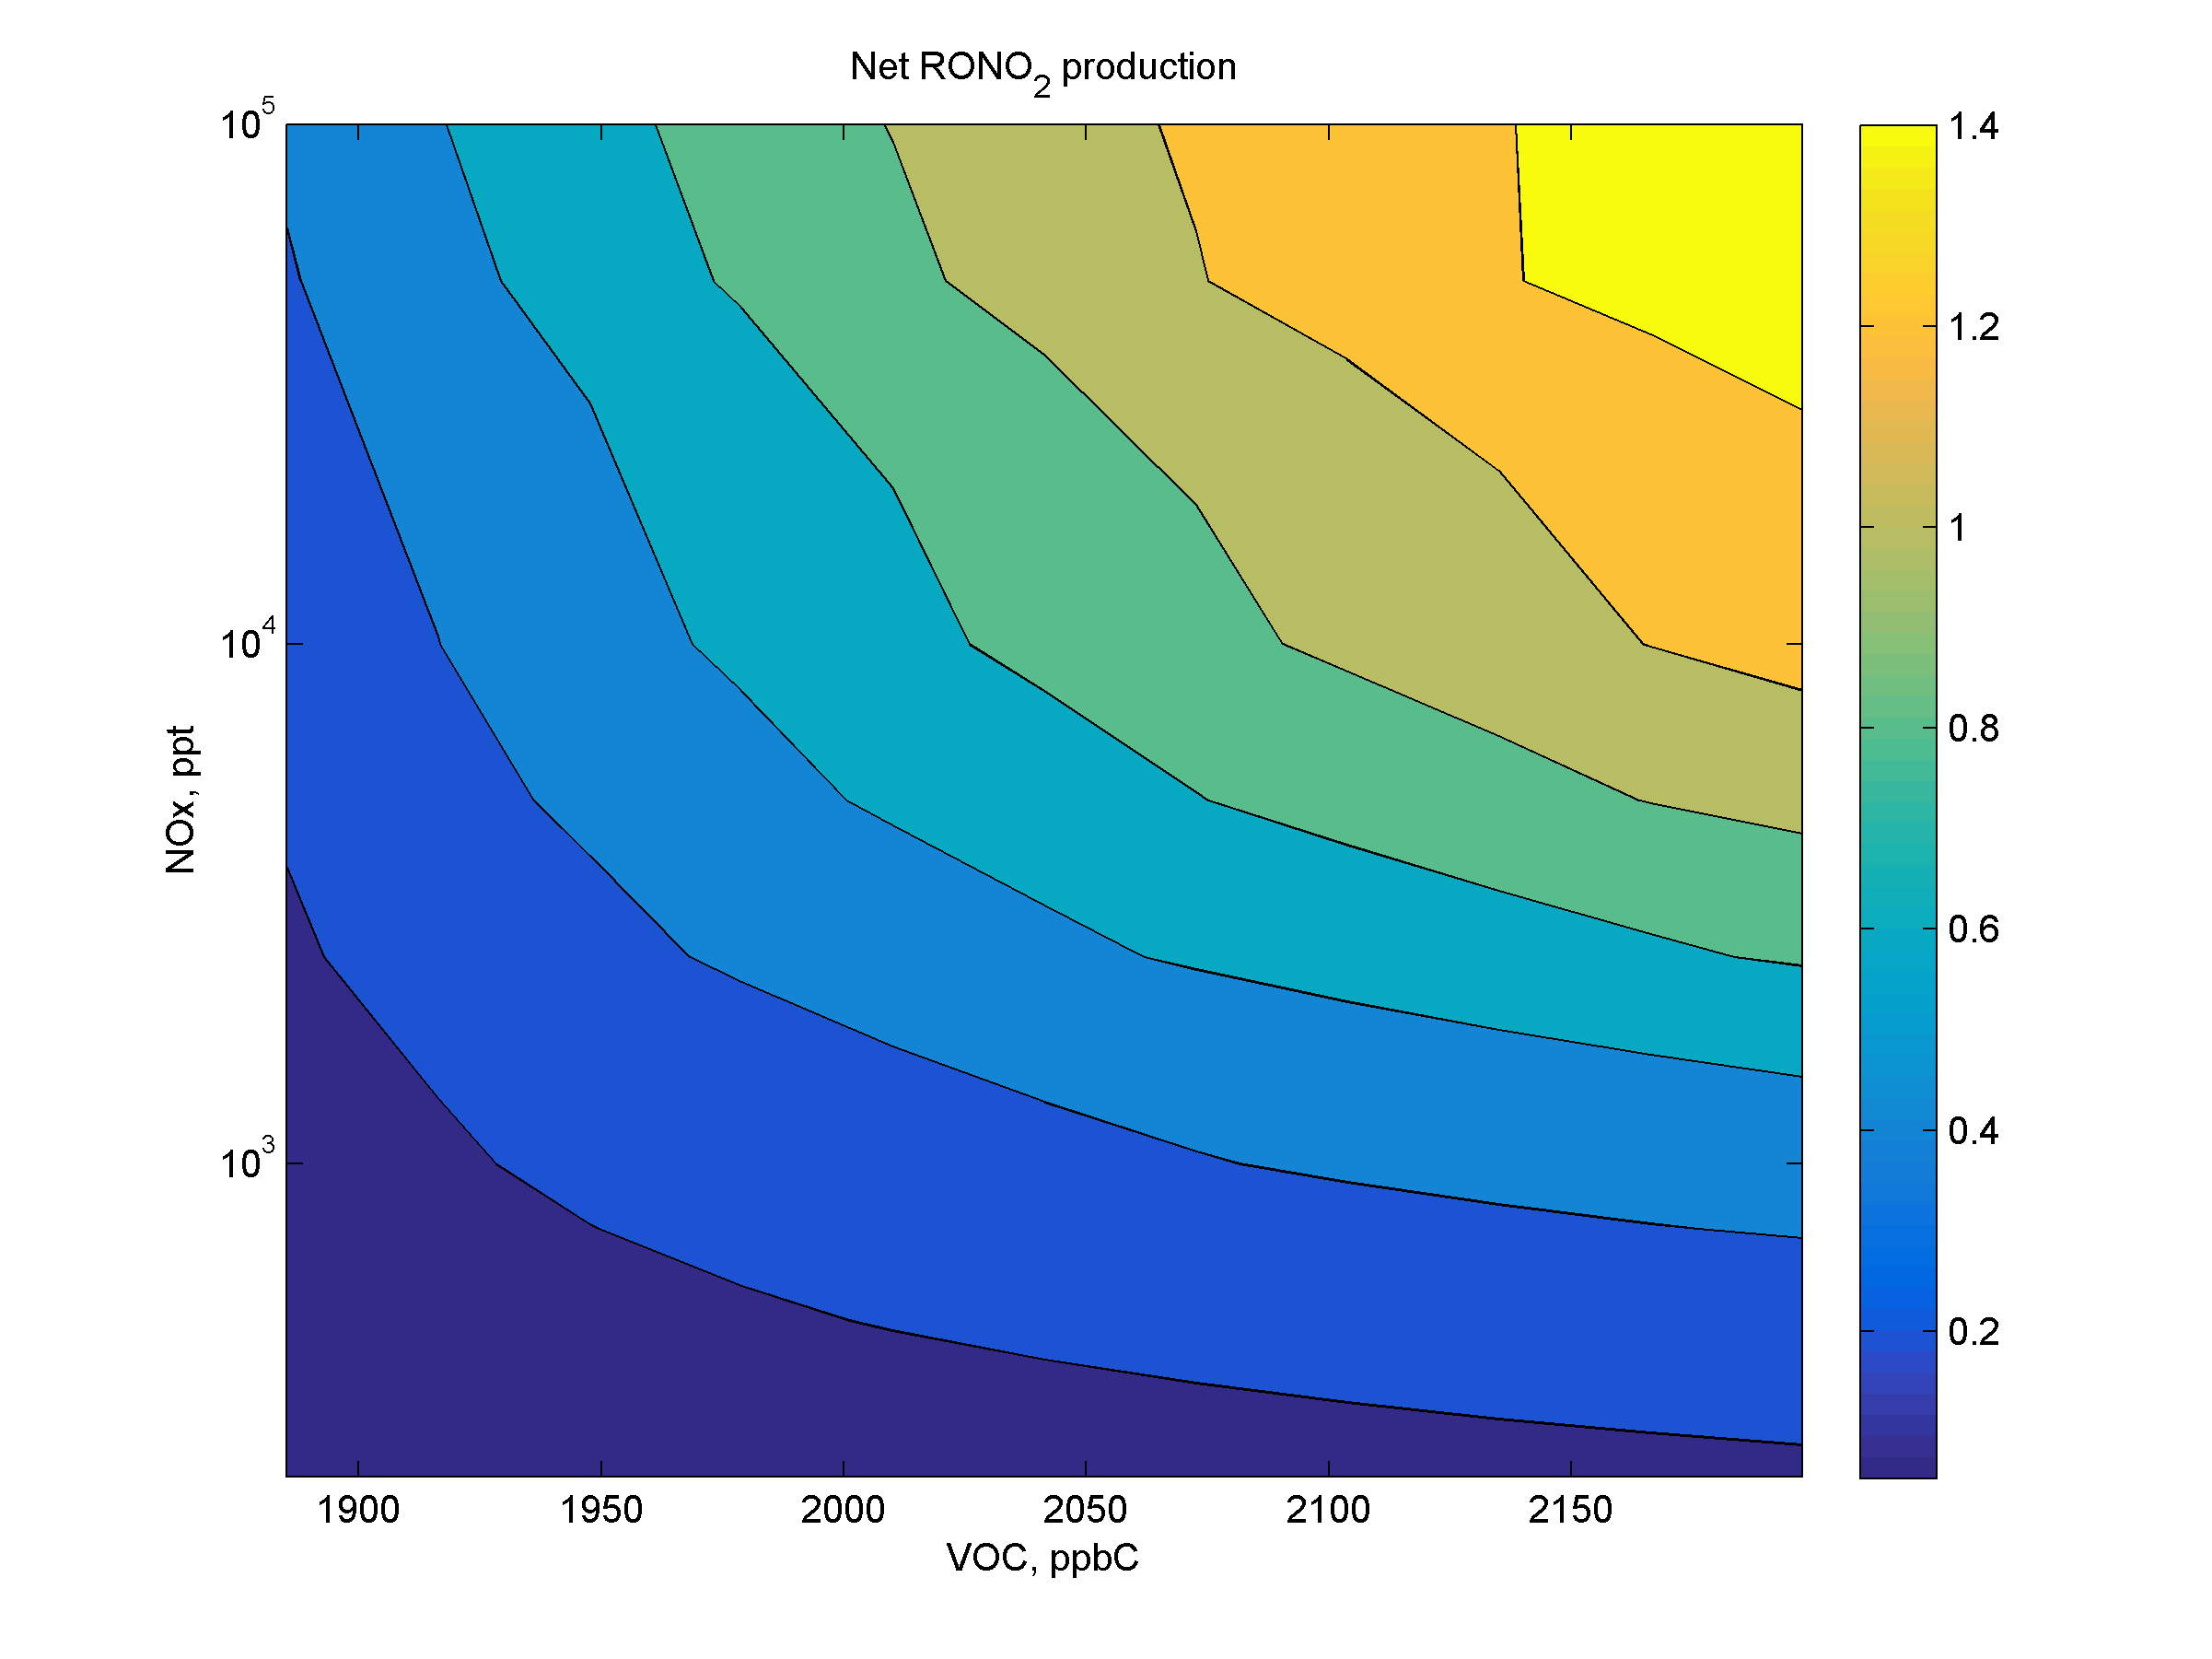
\includegraphics[width=.5\linewidth]{D:/FACSIMILE/ANsCBmodel/matlab/ANsCB_pics/ANsNOxVOC/allAN/chem_allAN_endtotalANs_noINORG_NOx_250ppt_100ppb.png}
\caption{Isopleths of net production of alkyl nitrates ($\Sigma RONO_2$) as a function of $NO_x$ and $VOCs$ levels.}\label{fig:endtotalANs}
\end{figure}

! Dependence of alkyl nitrate yield on carbon number (paper about n-alkanes): bigger yield of ANs from larger carbon number means that the potential for contributing to photochemical air pollution may be less for the larger (C>6) n-alkanes that for the smaller ones.

\subsection{$O_3$ production and carbon bonds}

\section{Discussion} \label{sec:discuss}
Future plans and possible improvements in the model.

The experimental results presented in the previous section provide an opportunity to speculate about the behaviour of our simple model of alkyl nitrate production and loss with time in comparison with the observational data. 

\section{Conclusion} \label{sec:conclusion}
\bibliography{diss_refs}

\section{Appendix I} \label{sec:appendix1}

\end{document}
